\documentclass[]{article}
\usepackage{lmodern}
\usepackage{amssymb,amsmath}
\usepackage{ifxetex,ifluatex}
\usepackage{fixltx2e} % provides \textsubscript
\ifnum 0\ifxetex 1\fi\ifluatex 1\fi=0 % if pdftex
  \usepackage[T1]{fontenc}
  \usepackage[utf8]{inputenc}
\else % if luatex or xelatex
  \ifxetex
    \usepackage{mathspec}
  \else
    \usepackage{fontspec}
  \fi
  \defaultfontfeatures{Ligatures=TeX,Scale=MatchLowercase}
\fi
% use upquote if available, for straight quotes in verbatim environments
\IfFileExists{upquote.sty}{\usepackage{upquote}}{}
% use microtype if available
\IfFileExists{microtype.sty}{%
\usepackage{microtype}
\UseMicrotypeSet[protrusion]{basicmath} % disable protrusion for tt fonts
}{}
\usepackage[margin=1in]{geometry}
\usepackage{hyperref}
\hypersetup{unicode=true,
            pdftitle={Laborator 5},
            pdfborder={0 0 0},
            breaklinks=true}
\urlstyle{same}  % don't use monospace font for urls
\usepackage{natbib}
\bibliographystyle{plainnat}
\usepackage{color}
\usepackage{fancyvrb}
\newcommand{\VerbBar}{|}
\newcommand{\VERB}{\Verb[commandchars=\\\{\}]}
\DefineVerbatimEnvironment{Highlighting}{Verbatim}{commandchars=\\\{\}}
% Add ',fontsize=\small' for more characters per line
\usepackage{framed}
\definecolor{shadecolor}{RGB}{248,248,248}
\newenvironment{Shaded}{\begin{snugshade}}{\end{snugshade}}
\newcommand{\KeywordTok}[1]{\textcolor[rgb]{0.13,0.29,0.53}{\textbf{#1}}}
\newcommand{\DataTypeTok}[1]{\textcolor[rgb]{0.13,0.29,0.53}{#1}}
\newcommand{\DecValTok}[1]{\textcolor[rgb]{0.00,0.00,0.81}{#1}}
\newcommand{\BaseNTok}[1]{\textcolor[rgb]{0.00,0.00,0.81}{#1}}
\newcommand{\FloatTok}[1]{\textcolor[rgb]{0.00,0.00,0.81}{#1}}
\newcommand{\ConstantTok}[1]{\textcolor[rgb]{0.00,0.00,0.00}{#1}}
\newcommand{\CharTok}[1]{\textcolor[rgb]{0.31,0.60,0.02}{#1}}
\newcommand{\SpecialCharTok}[1]{\textcolor[rgb]{0.00,0.00,0.00}{#1}}
\newcommand{\StringTok}[1]{\textcolor[rgb]{0.31,0.60,0.02}{#1}}
\newcommand{\VerbatimStringTok}[1]{\textcolor[rgb]{0.31,0.60,0.02}{#1}}
\newcommand{\SpecialStringTok}[1]{\textcolor[rgb]{0.31,0.60,0.02}{#1}}
\newcommand{\ImportTok}[1]{#1}
\newcommand{\CommentTok}[1]{\textcolor[rgb]{0.56,0.35,0.01}{\textit{#1}}}
\newcommand{\DocumentationTok}[1]{\textcolor[rgb]{0.56,0.35,0.01}{\textbf{\textit{#1}}}}
\newcommand{\AnnotationTok}[1]{\textcolor[rgb]{0.56,0.35,0.01}{\textbf{\textit{#1}}}}
\newcommand{\CommentVarTok}[1]{\textcolor[rgb]{0.56,0.35,0.01}{\textbf{\textit{#1}}}}
\newcommand{\OtherTok}[1]{\textcolor[rgb]{0.56,0.35,0.01}{#1}}
\newcommand{\FunctionTok}[1]{\textcolor[rgb]{0.00,0.00,0.00}{#1}}
\newcommand{\VariableTok}[1]{\textcolor[rgb]{0.00,0.00,0.00}{#1}}
\newcommand{\ControlFlowTok}[1]{\textcolor[rgb]{0.13,0.29,0.53}{\textbf{#1}}}
\newcommand{\OperatorTok}[1]{\textcolor[rgb]{0.81,0.36,0.00}{\textbf{#1}}}
\newcommand{\BuiltInTok}[1]{#1}
\newcommand{\ExtensionTok}[1]{#1}
\newcommand{\PreprocessorTok}[1]{\textcolor[rgb]{0.56,0.35,0.01}{\textit{#1}}}
\newcommand{\AttributeTok}[1]{\textcolor[rgb]{0.77,0.63,0.00}{#1}}
\newcommand{\RegionMarkerTok}[1]{#1}
\newcommand{\InformationTok}[1]{\textcolor[rgb]{0.56,0.35,0.01}{\textbf{\textit{#1}}}}
\newcommand{\WarningTok}[1]{\textcolor[rgb]{0.56,0.35,0.01}{\textbf{\textit{#1}}}}
\newcommand{\AlertTok}[1]{\textcolor[rgb]{0.94,0.16,0.16}{#1}}
\newcommand{\ErrorTok}[1]{\textcolor[rgb]{0.64,0.00,0.00}{\textbf{#1}}}
\newcommand{\NormalTok}[1]{#1}
\usepackage{graphicx,grffile}
\makeatletter
\def\maxwidth{\ifdim\Gin@nat@width>\linewidth\linewidth\else\Gin@nat@width\fi}
\def\maxheight{\ifdim\Gin@nat@height>\textheight\textheight\else\Gin@nat@height\fi}
\makeatother
% Scale images if necessary, so that they will not overflow the page
% margins by default, and it is still possible to overwrite the defaults
% using explicit options in \includegraphics[width, height, ...]{}
\setkeys{Gin}{width=\maxwidth,height=\maxheight,keepaspectratio}
\IfFileExists{parskip.sty}{%
\usepackage{parskip}
}{% else
\setlength{\parindent}{0pt}
\setlength{\parskip}{6pt plus 2pt minus 1pt}
}
\setlength{\emergencystretch}{3em}  % prevent overfull lines
\providecommand{\tightlist}{%
  \setlength{\itemsep}{0pt}\setlength{\parskip}{0pt}}
\setcounter{secnumdepth}{5}
% Redefines (sub)paragraphs to behave more like sections
\ifx\paragraph\undefined\else
\let\oldparagraph\paragraph
\renewcommand{\paragraph}[1]{\oldparagraph{#1}\mbox{}}
\fi
\ifx\subparagraph\undefined\else
\let\oldsubparagraph\subparagraph
\renewcommand{\subparagraph}[1]{\oldsubparagraph{#1}\mbox{}}
\fi

%%% Use protect on footnotes to avoid problems with footnotes in titles
\let\rmarkdownfootnote\footnote%
\def\footnote{\protect\rmarkdownfootnote}

%%% Change title format to be more compact
\usepackage{titling}

% Create subtitle command for use in maketitle
\newcommand{\subtitle}[1]{
  \posttitle{
    \begin{center}\large#1\end{center}
    }
}

\setlength{\droptitle}{-2em}
  \title{Laborator 5}
  \pretitle{\vspace{\droptitle}\centering\huge}
  \posttitle{\par}
\subtitle{Compararea proporțiilor și tabele de contingență}
  \author{}
  \preauthor{}\postauthor{}
  \date{}
  \predate{}\postdate{}

\usepackage{booktabs}
\usepackage{longtable}
\usepackage{framed,color}
\definecolor{shadecolor}{RGB}{248, 248, 248}
%\definecolor{shadecolor1}{RGB}{216,225,235}
%\definecolor{framecolor}{RGB}{108,123,13}

%\definecolor{shadecolor}{RGB}{226, 255, 241}
\definecolor{shadecolor1}{RGB}{217,225,199}
\definecolor{framecolor}{RGB}{60,179,113}

\ifxetex
  \usepackage{letltxmacro}
  \setlength{\XeTeXLinkMargin}{1pt}
  \LetLtxMacro\SavedIncludeGraphics\includegraphics
  \def\includegraphics#1#{% #1 catches optional stuff (star/opt. arg.)
    \IncludeGraphicsAux{#1}%
  }%
  \newcommand*{\IncludeGraphicsAux}[2]{%
    \XeTeXLinkBox{%
      \SavedIncludeGraphics#1{#2}%
    }%
  }%
\fi

\newenvironment{frshaded*}{%
  \def\FrameCommand{\fboxrule=\FrameRule\fboxsep=\FrameSep \fcolorbox{framecolor}{shadecolor1}}%
  \MakeFramed {\advance\hsize-\width \FrameRestore}}%
{\endMakeFramed}

\newenvironment{rmdblock}[1]
  {\begin{frshaded*}
  \begin{itemize}
  \renewcommand{\labelitemi}{
    \raisebox{-.7\height}[0pt][0pt]{
      {\setkeys{Gin}{width=2em,keepaspectratio}\includegraphics{images/icons/#1}}
    }
  }
  \item
  }
  {
  \end{itemize}
  \end{frshaded*}
  }

\newenvironment{rmdcaution}
  {\begin{rmdblock}{caution}}
  {\end{rmdblock}}
% \newenvironment{rmdinsight}
%   {\begin{rmdblock}{insight}}
%   {\end{rmdblock}}
\newenvironment{rmdexercise}
  {\begin{rmdblock}{exercise}}
  {\end{rmdblock}}
\newenvironment{rmdtip}
  {\begin{rmdblock}{tip}}
  {\end{rmdblock}}

%%%%%%%%%%%%%%%%%%%%%%%%%%%%%%%%%%%%%%%%%%%%%%%%%%%%%%%%%
%\usepackage{hyperref}
%\hypersetup{unicode=true,
%            pdftitle={Curs Biostatistica 2018},
%            pdfauthor={Alexandru Amarioarei},
%            pdfborder={0 0 0},
%            colorlinks,%
%            citecolor=green,%
%            filecolor=green,%
%            linkcolor=green,%
%            urlcolor=green}
%\urlstyle{same}

%%%%%%%%%%%%%%%%%%%%%%%%%%%%%%%%%%%%%%%%%%%%%%%%%%%%%%%%%%%%%%%%%%%%%%%%%%%%%%%%%%%%%%%%%%%%%%%%%%%%%%%%%%%%%%%%%%%%%
%%%%%%%%%%% For insight block %%%%%%%%%%%%%%%%%%%%%%%%%%
\definecolor{shadecolor_insight}{RGB}{223,240,216}
\definecolor{framecolor_insight}{RGB}{136,193,137}

%\definecolor{shadecolor_insight}{RGB}{217,225,199}
%\definecolor{framecolor_insight}{RGB}{60,179,113}

\newenvironment{frshaded_insight*}{%
  \def\FrameCommand{\fboxrule=\FrameRule\fboxsep=\FrameSep \fcolorbox{framecolor_insight}{shadecolor_insight}}%
  \MakeFramed {\advance\hsize-\width \FrameRestore}}%
{\endMakeFramed}

\newenvironment{rmdblock_insight}[1]
  {\begin{frshaded_insight*}
  \begin{itemize}
  \renewcommand{\labelitemi}{
    \raisebox{-.7\height}[0pt][0pt]{
      {\setkeys{Gin}{width=2em,keepaspectratio}\includegraphics{images/icons/#1}}
    }
  }
  \item
  }
  {
  \end{itemize}
  \end{frshaded_insight*}
  }

\newenvironment{rmdinsight}
  {\begin{rmdblock_insight}{insight}}
  {\end{rmdblock_insight}}

%%%%%%%%%%%%%%%%%%%%%%%%%%%%%%%%%%%%%%%%%%%%%%%%%%%%%%%%%%%%%%%%%%%%%%%%%%%%%%%%%%%%%%%%%%%%%%%%%%%%%%%%%%%%%%%%%%%%%
\usepackage{subfigure}
\usepackage{booktabs}
\usepackage{slashbox}
\usepackage{color}
%%%%%%%%%%%%%%%%%%%%%%%%%%%%%%%%%%%%%%%%%
\definecolor{linkcol}{rgb}{0,0,0.4}
\definecolor{citecol}{rgb}{0.5,0,0}

% Change this to change the informations included in the pdf file
% \usepackage[pagebackref]{hyperref}
% \usepackage[verbose]{backref}
% \backrefsetup{verbose=false}
\usepackage[hyperpageref]{backref}
% \PassOptionsToPackage{pagebackref}{hyperref}
% See hyperref documentation for information on those parameters

\hypersetup
{
bookmarksopen=true,
pdftitle="Curs Biostatistica",
pdfauthor="Alexandru Amarioarei",
pdfsubject="Laboratoare Biostatistica", %subject of the document
pdfmenubar=true, %menubar shown
pdfhighlight=/O, %effect of clicking on a link
colorlinks=true, %couleurs sur les liens hypertextes
pdfpagemode=None, %aucun mode de page
pdfpagelayout=SinglePage, %ouverture en simple page
pdffitwindow=true, %pages ouvertes entierement dans toute la fenetre
linkcolor=linkcol, %couleur des liens hypertextes internes
citecolor=citecol, %couleur des liens pour les citations
urlcolor=linkcol %couleur des liens pour les url
}


% set the back references
\renewcommand*{\backref}[1]{}
\renewcommand*{\backreftwosep}{ și~} % inserted between entries 
                              % in a list of two entries, 
                              % default is " and~".
\renewcommand*{\backreflastsep}{, și~} % inserted between the last 
                               % two entries of a list with more
                               % than two entries, default is ", and~".
\renewcommand*{\backrefalt}[4]{%
    \ifcase #1 (Necitat.)%
    \or        (Citat la pagina~#2.)%
    \else      (Citat la paginile~#2.)%
    \fi}


%%%%%%%%%%%%%%%%%%%%%%%%%%%%%%%%%%%%%%%%%%%%%%%%%%%%%%%%%%%%%%%%%%%%%%%%%%%%%%%%%%%%%%%%%%%%%%%%%%%%%%%%%%%%%%%%%%%%%
%CITEVA DEFINITII
\def\om{\omega}
\def\Om{\Omega}
\def\et{\eta}
\def\td{\tilde{\delta}}
\def\m{{\mu}}
\def\n{{\nu}}
\def\k{{\kappa}}
\def\l{{\lambda}}
\def\L{{\Lambda}}
\def\g{{\gamma}}
\def\a{{\alpha}}
\def\e{{\varepsilon}}
\def\b{{\beta}}
\def\G{{\Gamma}}
\def\d{{\delta}}
\def\D{{\Delta}}
\def\t{{\theta}}
\def\s{{\sigma}}
\def\S{{\Sigma}}
\def\z{{\zeta}}
\def\qed{\hfill\Box}
\def\ds{\displaystyle}
\def\mc{\mathcal}
%%%%%%%%%%%%%%%%%%%%%%%%%%%%%%%%%%%%%%%%%%%%%%%%%%%%%%%%%%%%%%%%%%%%%%%%%%%%%%%%%%%%%%%%%%%%%%%%%%%%%%%%%%%%%%%%%%%%%%
\def\1{{\mathbf 1}}
\def\CC{{\mathbb C}}
\def\VV{{\mathbb V}}
\def\RR{{\mathbb R}}
\def\QQ{{\mathbb Q}}
\def\ZZ{{\mathbb Z}}
\def\PP{{\mathbb P}}
\def\EE{{\mathbb E}}
\def\NN{{\mathbb N}}
\def\FF{{\mathbb F}}
%\def\SS{{\mathbb S}}
\def\MA{{\mathcal A}}
\def\MO{{\mathcal O}}
\def\MF{{\mathcal F}}
\def\ME{{\mathcal E}}
\def\MR{{\mathcal R}}
\def\MB{{\mathcal B}}
\def\MM{{\mathcal M}}
\def\MN{{\mathcal N}}
\def\MU{{\mathcal U}}
\def\MP{{\mathcal P}}
\def\MS{{\mathcal S}}
\def\MBS{{\mathbf S}}
\def\MX{{\bm{ \mathscr X}}}

% independent sign
\newcommand\independent{\protect\mathpalette{\protect\independenT}{\perp}}
\def\independenT#1#2{\mathrel{\rlap{$#1#2$}\mkern2mu{#1#2}}}

\renewcommand\tablename{Tab.}
\renewcommand{\figurename}{Fig.}
\renewcommand\refname{Referințe}

%%%%%%%%%%%%%%%%%%%%%%%%%%%%%%%%%%%%%%%%%%%%%%%%%%%%%%%%%%%%%%%%%%%%%%%%%%%%%%%%%%%%%%%%%%%%%%%%%%%%%%%%%%%%%%%%%%%%%
%Header and Footer
\usepackage{fancyhdr}

\pagestyle{fancy}
\fancyhf{}
\rhead{Universitatea din Bucure\c sti\\ Facultatea de Matematic\u a \c si Informatic\u a}
\lhead{\textit{Curs}: Biostatistic\u a 2018\\ \textit{Instructor}: A. Am\u arioarei}
\rfoot{Pagina \thepage}
\lfoot{Grupa: 503}
%%%%%%%%%%%%%%%%%%%%%%%%%%%%%%%%%%%%%%%
\usepackage{booktabs}
\usepackage{longtable}
\usepackage{array}
\usepackage{multirow}
\usepackage[table]{xcolor}
\usepackage{wrapfig}
\usepackage{float}
\usepackage{colortbl}
\usepackage{pdflscape}
\usepackage{tabu}
\usepackage{threeparttable}
\usepackage{threeparttablex}
\usepackage[normalem]{ulem}
\usepackage{makecell}

\begin{document}
\maketitle

%%%%%%%%%%%%%%%%%%%%%%%%
\thispagestyle{fancy}

Obiectivul acestui laborator este de a prezenta câteva teste statistice
folosite pentru testarea ipotezelor statistice atunci când datele sunt
de tip categoric.

\section{\texorpdfstring{Compararea proporțiilor și tabele de
contingență
\(2\times 2\)}{Compararea proporțiilor și tabele de contingență 2\textbackslash{}times 2}}\label{compararea-proportiilor-si-tabele-de-contingenta-2times-2}

Considerăm următorul exemplu:

\begin{rmdexercise}
Un studiu clinic a investigat efectele metodelor contraceptive orale
(OC) asupra bolilor de inimă la femeile cu vârste între 40 și 44 de ani.
Cercetătorii au găsit că printre 5000 de femei care utilizau metode
contraceptive orale la momentul studiului (cazuri), 13 dintre acestea au
dezvoltat un infarct miocardic (MI) (pe o perioadă de 3 ani) pe când
printre 10000 de femei care nu au folosit niciodată OC (grupul de
control) doar 7 au dezvoltat MI (pe aceeași perioadă). Vrem să vedem
dacă există vreo asociere între consumul de anticoncepționale pe cale
orală și incidența infarctului miocardic (pe această perioadă).
\end{rmdexercise}

Fie \(\pi_1=\mathbb{P}(MI\,|\,OC)\), probabilitatea ca femeile să
dezvolte infarct miocardic (MI) în cazul grupului care a consumat
contraceptive orale (OC) și \(\pi_2=\mathbb{P}(MI\,|\,non-OC)\),
probabilitatea ca femeile să dezvolte infarct miocardic (MI) în cazul
grupului care nu a consumat contraceptive orale (OC). Întrebarea este
dacă probabilitatea de a face infarct miocardic diferă între cele două
grupuri (cazuri vs control). Cu alte cuvinte vrem să testăm ipotezele
statistice:

\[
  \begin{array}{ll}
    H_0:\,\,\pi_1=\pi_2\\
    H_1:\,\,\pi_1\neq \pi_2
  \end{array}
\]

\subsection{Compararea proporțiilor prin aproximarea
normală}\label{compararea-proportiilor-prin-aproximarea-normala}

Putem modela problema astfel: considerăm
\(X_1, X_2, \ldots, X_{n_1}\in\{0,1\}\) (\(0\) - nu a dezvoltat infarct
miocardic, \(1\) - a dezvoltat infarct miocardic pe perioada studiului)
un eșantion de talie \(n_1\) (\(n_1 = 5000\)) dintr-o populație
Bernoulli \(\mathcal{B}(\pi_1)\) care să reprezinte populația femeilor
cu vârste între 40 și 44 de ani care au consumat contraceptive orale
(cazuri) și respectiv un eșantion
\(Y_1, Y_2, \ldots, Y_{n_2}\in\{0,1\}\) un eșantion de talie \(n_2\)
(\(n_2 = 10000\)) dintr-o populație Bernoulli \(\mathcal{B}(\pi_2)\)
care să reprezinte populația femeilor cu vârste între 40 și 44 de ani
care nu au consumat contraceptive orale (control). Vom presupune că
eșantioanele sunt suficient de mari pentru a putea aplica aproximarea
normală a binomialei (e.g.~vezi
\href{https://alexamarioarei.github.io/Teaching/2017-2018/PS\%20web\%20page/labs/Lab_4.html\#3_aproximarea_poisson_\%C8\%99i_normal\%C4\%83_a_binomialei}{aici}).

Se poate verifica cu ușurință că sub \(H_0:\,\pi_1=\pi_2=\pi\) are loc

\[
  \hat{\pi}_1 - \hat{\pi}_2\sim\mathcal{N}\left(\underbrace{\pi_1-\pi_2}_{=0}, \pi(1-\pi)\left(\frac{1}{n_1} + \frac{1}{n_2}\right)\right)
\]

unde \(\hat{\pi}_1 = \bar{X}_{n_1}\) iar
\(\hat{\pi}_2 = \bar{Y}_{n_2}\). Astfel, sub \(H_0\), avem

\[
  Z = \frac{\hat{\pi}_1 - \hat{\pi}_2}{\sqrt{\pi(1-\pi)\left(\frac{1}{n_1} + \frac{1}{n_2}\right)}} \sim \mathcal{N}(0,1)
\]

și cum \(\pi\) este necunoscut putem să-l aproximăm din cele două
eșantioane luate împreună (estimatorul \emph{pooled})

\[
  \hat{\pi} = \frac{\sum_{i = 1}^{n_1}X_i + \sum_{j = 1}^{n_2}Y_j}{n_1+n_2} = \frac{n_1\hat{\pi}_1 + n_2\hat{\pi}_2}{n_1+n_2}.
\]

Dacă luăm în calcul corecția de continuitate a aproximării normale a
binomialei atunci regiunea critică a testului bilateral de nivel
\(\alpha\) (acest test se numește \emph{testul de scor} și este
recomandat atunci când vrem să comparîăm proporții în locul
\emph{testului lui Wald}), cu ipotezele statistice
\(H_0:\,\pi_1=\pi_2\,\,vs\,\,H_1:\,\pi_1\neq \pi_2\), este

\[
  C = \left\{(x_1,\ldots,x_{n_1},y_1,\ldots,y_{n_2})\,|\,\frac{|\hat{\pi}_1 - \hat{\pi}_2| - \frac{1}{2}\left(\frac{1}{n_1} + \frac{1}{n_2}\right)}{\sqrt{\hat{\pi}(1-\hat{\pi})\left(\frac{1}{n_1} + \frac{1}{n_2}\right)}}>z_{1-\frac{\alpha}{2}}\right\}
\]

iar p-valoarea aproximativă a testului este

\[
  p-val = 2(1-\Phi(z_{\text{obs}})).
\]

De regulă, în practică, putem folosi aproximarea normală a binomialei și
testul de comparare a proporțiilor cu regiunea critică \(C\) atunci când
sunt îndeplinite condițiile \(n_1\hat{\pi}(1-\hat{\pi})\geq 5\) și
\(n_2\hat{\pi}(1-\hat{\pi})\geq 5\).

În R avem

\begin{Shaded}
\begin{Highlighting}[]
\NormalTok{n1 =}\StringTok{ }\DecValTok{5000} \CommentTok{# nr total cazuri OC}
\NormalTok{n11 =}\StringTok{ }\DecValTok{13} \CommentTok{# nr cazuri cu MI}

\NormalTok{n2 =}\StringTok{ }\DecValTok{10000} \CommentTok{# nr total control non-OC}
\NormalTok{n21 =}\StringTok{ }\DecValTok{7} \CommentTok{# nr control cu MI}

\NormalTok{p1 =}\StringTok{ }\NormalTok{n11}\OperatorTok{/}\NormalTok{n1}
\NormalTok{p2 =}\StringTok{ }\NormalTok{n21}\OperatorTok{/}\NormalTok{n2}

\NormalTok{p =}\StringTok{ }\NormalTok{(n11}\OperatorTok{+}\NormalTok{n21)}\OperatorTok{/}\NormalTok{(n1}\OperatorTok{+}\NormalTok{n2) }\CommentTok{# proportia comuna - pooled p}
\end{Highlighting}
\end{Shaded}

și putem verifica cele două condiții de aplicabilitate a aproximării
normale

\begin{Shaded}
\begin{Highlighting}[]
\CommentTok{# Verificam daca putem aplica aproximarea normala }
\NormalTok{n1}\OperatorTok{*}\NormalTok{p}\OperatorTok{*}\NormalTok{(}\DecValTok{1}\OperatorTok{-}\NormalTok{p)}\OperatorTok{>}\DecValTok{5}
\NormalTok{[}\DecValTok{1}\NormalTok{] }\OtherTok{TRUE}
\NormalTok{n2}\OperatorTok{*}\NormalTok{p}\OperatorTok{*}\NormalTok{(}\DecValTok{1}\OperatorTok{-}\NormalTok{p)}\OperatorTok{>}\DecValTok{5}
\NormalTok{[}\DecValTok{1}\NormalTok{] }\OtherTok{TRUE}
\end{Highlighting}
\end{Shaded}

Calculul statisticii de test și a p-valorii testului, pentru exemplul
nostru, sunt

\begin{Shaded}
\begin{Highlighting}[]
\CommentTok{# Calculam statistica de test cu corectia de continuitate}
\NormalTok{z =}\StringTok{ }\NormalTok{(}\KeywordTok{abs}\NormalTok{(p1}\OperatorTok{-}\NormalTok{p2)}\OperatorTok{-}\FloatTok{0.5}\OperatorTok{*}\NormalTok{(}\DecValTok{1}\OperatorTok{/}\NormalTok{n1}\OperatorTok{+}\DecValTok{1}\OperatorTok{/}\NormalTok{n2))}\OperatorTok{/}\KeywordTok{sqrt}\NormalTok{(p}\OperatorTok{*}\NormalTok{(}\DecValTok{1}\OperatorTok{-}\NormalTok{p)}\OperatorTok{*}\NormalTok{(}\DecValTok{1}\OperatorTok{/}\NormalTok{n1}\OperatorTok{+}\DecValTok{1}\OperatorTok{/}\NormalTok{n2))}
\NormalTok{z}
\NormalTok{[}\DecValTok{1}\NormalTok{] }\FloatTok{2.768839}

\CommentTok{# Calcul de p-valoare: test bilateral}
\NormalTok{pval =}\StringTok{ }\KeywordTok{min}\NormalTok{(}\DecValTok{2}\OperatorTok{*}\NormalTok{(}\DecValTok{1}\OperatorTok{-}\KeywordTok{pnorm}\NormalTok{(z)), }\DecValTok{1}\NormalTok{)}
\NormalTok{pval}
\NormalTok{[}\DecValTok{1}\NormalTok{] }\FloatTok{0.005625635}
\end{Highlighting}
\end{Shaded}

Observăm că același răspuns se obține și dacă folosim funcția
\texttt{prop.test()} din R:

\begin{Shaded}
\begin{Highlighting}[]
\KeywordTok{prop.test}\NormalTok{(}\KeywordTok{c}\NormalTok{(}\DecValTok{13}\NormalTok{, }\DecValTok{7}\NormalTok{), }\KeywordTok{c}\NormalTok{(}\DecValTok{5000}\NormalTok{, }\DecValTok{10000}\NormalTok{))}

    \DecValTok{2}\OperatorTok{-}\NormalTok{sample test }\ControlFlowTok{for}\NormalTok{ equality of proportions with continuity}
\NormalTok{    correction}

\NormalTok{data}\OperatorTok{:}\StringTok{  }\KeywordTok{c}\NormalTok{(}\DecValTok{13}\NormalTok{, }\DecValTok{7}\NormalTok{) out of }\KeywordTok{c}\NormalTok{(}\DecValTok{5000}\NormalTok{, }\DecValTok{10000}\NormalTok{)}
\NormalTok{X}\OperatorTok{-}\NormalTok{squared =}\StringTok{ }\FloatTok{7.6665}\NormalTok{, df =}\StringTok{ }\DecValTok{1}\NormalTok{, p}\OperatorTok{-}\NormalTok{value =}\StringTok{ }\FloatTok{0.005626}
\NormalTok{alternative hypothesis}\OperatorTok{:}\StringTok{ }\NormalTok{two.sided}
\DecValTok{95}\NormalTok{ percent confidence interval}\OperatorTok{:}
\StringTok{ }\FloatTok{0.0002463116} \FloatTok{0.0035536884}
\NormalTok{sample estimates}\OperatorTok{:}
\NormalTok{prop }\DecValTok{1}\NormalTok{ prop }\DecValTok{2} 
\FloatTok{0.0026} \FloatTok{0.0007} 
\end{Highlighting}
\end{Shaded}

De asemenea putem construi și intervalul de încredere de nivel
\(1-\alpha\), corespunzător

\begin{verbatim}
IC pentru pi1-pi2 la pragul de semnificatie 95% este 
 IC = [ 0.0006612366 , 0.003138763 ]
\end{verbatim}

precum și intervalul de încredere clasic pentru diferența proporțiilor,
obținut prin aproximarea lui Wald

\[
  \hat{\pi}_1 - \hat{\pi}_2 \pm z_{1-\frac{\alpha}{2}}\sqrt{\frac{\hat{\pi}_1(1-\hat{\pi}_1)}{n_1} + \frac{\hat{\pi}_2(1-\hat{\pi}_2)}{n_2}}
\]

\begin{verbatim}
IC pentru pi1-pi2 la pragul de semnificatie 95% este 
 IC = [ 0.0003963116 , 0.003403688 ]
\end{verbatim}

În articolul \citep{Agresti2000}, autorii prezintă un alt interval de
încredere (ajustat prin adăugarea a două observații la fiecare eșantion,
un \(1\) și un \(0\)) pentru diferența proporțiilor

\[
  \bar{\pi}_1 - \bar{\pi}_2 \pm z_{1-\frac{\alpha}{2}}\sqrt{\frac{\bar{\pi}_1(1-\bar{\pi}_1)}{n_1+2} + \frac{\bar{\pi}_2(1-\bar{\pi}_2)}{n_2+2}}
\]

unde \(\bar{\pi}_1 = \frac{\sum_{i = 1}^{n_1}X_i + 1}{n_1+2}\) iar
\(\bar{\pi}_2 = \frac{\sum_{j = 1}^{n_1}Y_j + 1}{n_2+2}\)

\begin{verbatim}
IC (Agresti-Caffo) pentru pi1-pi2 la pragul de semnificatie 95% este 
 IC = [ 0.0006853283 , 0.003312753 ]
\end{verbatim}

\begin{center}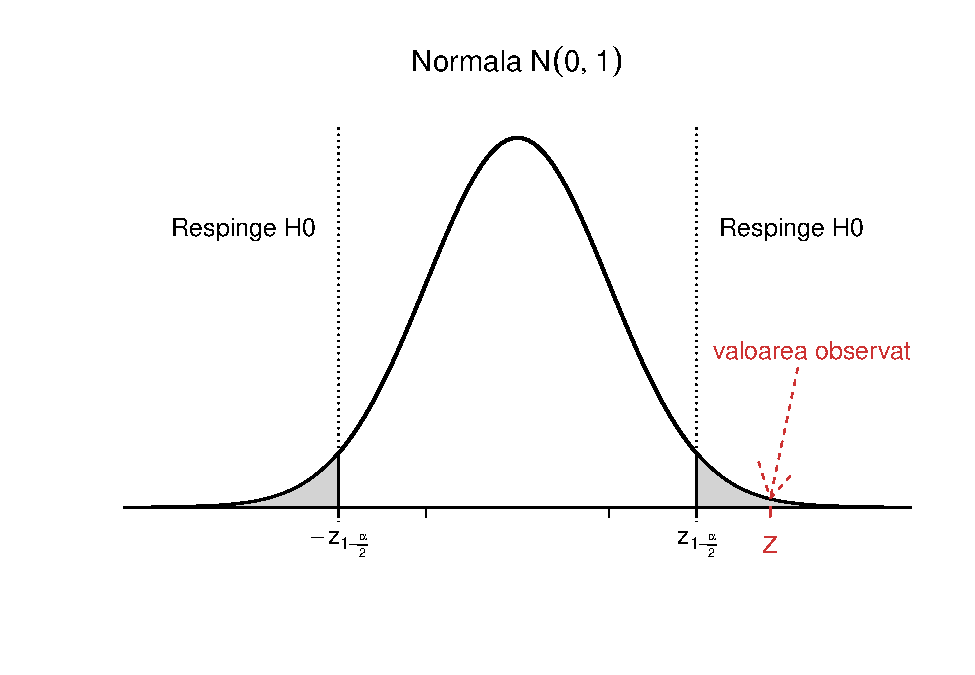
\includegraphics[width=0.8\linewidth]{Lab_5_files/figure-latex/unnamed-chunk-10-1} \end{center}

Concluzionăm că folosirea de anticoncepționale pe cale orală este
semnificativ asociată cu incidența crescută de cazuri de MI la femeile
cu vârste între 40 și 44 de ani pe perioada de 3 ani a studiului.

\begin{rmdexercise}
Puteți crea o funcție care să automatizeze procesul ?
\end{rmdexercise}

\subsection{\texorpdfstring{Metoda tabelelor de contingență și testul
\(\chi^2\) al lui
Pearson}{Metoda tabelelor de contingență și testul \textbackslash{}chi\^{}2 al lui Pearson}}\label{metoda-tabelelor-de-contingenta-si-testul-chi2-al-lui-pearson}

Rescriem problema de mai sus sub formă de tabel de contingență
\(2\times2\) (un tabel în care datele apar clasificate după valorile a
două variabile categorice, cu două clase fiecare) pentru vectorul
aleator
\((X,Y)\in\{a_1, a_2\}\times\{b_1,b_2\} = \{\text{OC}, \text{non-OC}\}\times\{\text{MI},\text{non-MI}\}\):

\[
  \begin{array}{c|c|c|c}
    X/Y & b_1 & b_2 & \text{Total}\\
    \hline
    a_1 & n_{11} & n_{12} & n_{1\cdot} = n_{11} + n_{12}\\
    \hline
    a_2 & n_{21} & n_{22} & n_{2\cdot} = n_{21} + n_{22}\\
    \hline
    \text{Total} & n_{\cdot 1} = n_{11} + n_{21} & n_{\cdot 2} = n_{12} + n_{22} & n = \sum_{i,j = 1}^{2}n_{ij}\\
  \end{array}
\] care în cazul problemei noastre este

\rowcolors{2}{gray!6}{white}

\begin{longtable}{lccccccccc}
\hiderowcolors
\toprule
  & MI & non-MI & Total\\
\midrule
\endfirsthead
\multicolumn{10}{@{}l}{\textit{(continued)}}\\
\toprule
  & MI & non-MI & Total\\
\midrule
\endhead
\
\endfoot
\bottomrule
\endlastfoot
\showrowcolors
OC & 13 & 4987 & 5000\\
non-OC & 7 & 9993 & 10000\\
Total & 20 & 14980 & 15000\\*
\end{longtable}

\rowcolors{2}{white}{white}

Acesta se mai numește și tabelul observat

\[
  \text{Tabel}_{obs} = \begin{array}{c|c}
      O_{11} & O_{12}\\
      \hline
      O_{21} & O_{22}
  \end{array} = \begin{array}{c|c}
      n_{11} & n_{12}\\
      \hline
      n_{21} & n_{22}
  \end{array}
\] Repartiția vectorului \((X,Y)\) este dată de
\(\mathbb{P}\circ (X,Y)^{-1} = \sum_{i = 1}^{2}\sum_{j = 1}^{2}p_{ij}\delta_{(a_i,b_j)}\),
unde \(\mathbb{P}((X,Y) = (a_i, b_j)) = p_{ij}\)

\[
  \begin{array}{c|c|c|c}
    X/Y & b_1 & b_2 & \sum\\
    \hline
    a_1 & p_{11} & p_{12} & p_1 = p_{11} + p_{12}\\
    \hline
    a_2 & p_{21} & p_{22} & p_2 = p_{21} + p_{22}\\
    \hline
    \sum & q_1 = p_{11} + p_{21} & q_2 = p_{12} + p_{22} & 1\\
  \end{array}
\]

iar repartițiile marginale sunt
\(\mathbb{P}\circ X^{-1} = \sum_{i = 1}^{2}p_{i}\delta_{a_i}\),
\(\mathbb{P}\circ Y^{-1} = \sum_{j = 1}^{2}q_{j}\delta_{b_j}\) cu
\(\mathbb{P}(X = a_i) = p_i\) și respectiv
\(\mathbb{P}(Y = b_j) = q_j\).

Suntem interesați în testarea ipotezelor

\[
H_0:\, \pi_1 = \pi_2\,\, vs \,\, H_1:\,\pi_1 \neq \pi_2
\]

unde \(\pi_1=\mathbb{P}(MI\,|\,OC) = \mathbb{P}(Y = b_1\,|\,X = a_1)\)
iar
\(\pi_2=\mathbb{P}(MI\,|\,non-OC) = \mathbb{P}(Y = b_1\,|\,X = a_2)\).
Observăm că

\[
  \pi_1 = \pi_2 \iff \frac{p_{11}}{p_1} = \frac{p_{21}}{p_2} \iff \frac{p_{11}}{p_1} = \frac{q_1 - p_{11}}{p_2} \iff p_{11} = p_1q_1
\] și, în mod similar, se poate verifica că \(p_{ij} = p_iq_j\),
\(\forall i,j\in\{1,2\}\). Cu alte cuvinte, ipoteza nulă se mai scrie și
sub forma

\[
  H_0:\, \{\pi_1 = \pi_2\} = \left\{p_{ij} = p_iq_j,\,\forall i,j\in\{1,2\}\right\}
\] Fie \((X_1, Y_1), (X_2, Y_2),\ldots,(X_n, Y_n)\) un eșantion de talie
\(n\) din populația \(\mathbb{P}\circ (X,Y)^{-1}\) și avem că
\(n_{ij} = \sum_{k = 1}^n\mathbf{1}_{(a_i, b_j)}(X_k, Y_k)\) (numărul de
observații din celula \((i,j)\)) iar
\(n_{i\cdot} = \sum_{j = 1}^{2}n_{ij}\),
\(n_{\cdot j} = \sum_{i = 1}^{2}n_{ij}\) și respectiv
\(n = \sum_{i,j = 1}^{2}n_{ij}\).

Sub ipoteza nulă, \(H_0\), avem că estimatorii de verosimilitate maximă
pentru \(p_i\) și \(q_j\) sunt

\[
  \hat{p}_i = \frac{n_{i\cdot}}{n},\,\, \hat{q}_j = \frac{n_{\cdot j}}{n}
\]

iar numărul de observații pe care ne așteptăm să-l observăm (sub
\(H_0\)) în fiecare celulă este

\[
  E_{ij} = n \hat{p}_{ij} \overset{H_0}{=} n \hat{p}_i \hat{q}_j = \frac{n_{i\cdot}n_{\cdot j}}{n}.
\] Astfel tabelul pe care ne așteptăm să-l observăm sub ipoteza nulă
este

\[
  \text{Tabel}_{exp} = \begin{array}{c|c}
      E_{11} & E_{12}\\
      \hline
      E_{21} & E_{22}
  \end{array} = \begin{array}{c|c}
      \frac{n_{1\cdot}n_{\cdot 1}}{n} & \frac{n_{1\cdot}n_{\cdot 2}}{n}\\
      \hline
      \frac{n_{2\cdot}n_{\cdot 1}}{n} & \frac{n_{2\cdot}n_{\cdot 2}}{n}
  \end{array}
\]

Calculul tabelului pe care ne așteptăm să-l observăm:

\begin{Shaded}
\begin{Highlighting}[]
\CommentTok{# Observat}
\NormalTok{n11 =}\StringTok{ }\DecValTok{13}
\NormalTok{n1o =}\StringTok{ }\DecValTok{5000}
\NormalTok{n12 =}\StringTok{ }\NormalTok{n1o}\OperatorTok{-}\NormalTok{n11}

\NormalTok{n21 =}\StringTok{ }\DecValTok{7}
\NormalTok{n2o =}\StringTok{ }\DecValTok{10000}
\NormalTok{n22 =}\StringTok{ }\NormalTok{n2o}\OperatorTok{-}\NormalTok{n21}

\NormalTok{no1 =}\StringTok{ }\NormalTok{n11}\OperatorTok{+}\NormalTok{n21}
\NormalTok{no2 =}\StringTok{ }\NormalTok{n12}\OperatorTok{+}\NormalTok{n22}

\NormalTok{n =}\StringTok{ }\NormalTok{n1o}\OperatorTok{+}\NormalTok{n2o}

\CommentTok{#Asteptat}
\NormalTok{e11 =}\StringTok{ }\NormalTok{n1o}\OperatorTok{*}\NormalTok{no1}\OperatorTok{/}\NormalTok{n}
\NormalTok{e12 =}\StringTok{ }\NormalTok{n1o}\OperatorTok{*}\NormalTok{no2}\OperatorTok{/}\NormalTok{n}
\NormalTok{e21 =}\StringTok{ }\NormalTok{n2o}\OperatorTok{*}\NormalTok{no1}\OperatorTok{/}\NormalTok{n}
\NormalTok{e22 =}\StringTok{ }\NormalTok{n2o}\OperatorTok{*}\NormalTok{no2}\OperatorTok{/}\NormalTok{n}

\NormalTok{Mobs =}\StringTok{ }\KeywordTok{matrix}\NormalTok{(}\KeywordTok{c}\NormalTok{(n11,n12,n21,n22),}\DataTypeTok{ncol =} \DecValTok{2}\NormalTok{, }\DataTypeTok{byrow =}\NormalTok{ T, }
              \DataTypeTok{dimnames =} \KeywordTok{list}\NormalTok{(}\KeywordTok{c}\NormalTok{(}\StringTok{"OC"}\NormalTok{,}\StringTok{"non-OC"}\NormalTok{), }\KeywordTok{c}\NormalTok{(}\StringTok{"MI"}\NormalTok{, }\StringTok{"non-MI"}\NormalTok{)))}

\NormalTok{Mexp =}\StringTok{ }\KeywordTok{matrix}\NormalTok{(}\KeywordTok{c}\NormalTok{(e11,e12,e21,e22),}\DataTypeTok{ncol =} \DecValTok{2}\NormalTok{, }\DataTypeTok{byrow =}\NormalTok{ T, }
              \DataTypeTok{dimnames =} \KeywordTok{list}\NormalTok{(}\KeywordTok{c}\NormalTok{(}\StringTok{"OC"}\NormalTok{,}\StringTok{"non-OC"}\NormalTok{), }\KeywordTok{c}\NormalTok{(}\StringTok{"MI"}\NormalTok{, }\StringTok{"non-MI"}\NormalTok{)))}
\end{Highlighting}
\end{Shaded}

\rowcolors{2}{gray!6}{white}

\begin{longtable}{lcccccc}
\hiderowcolors
\toprule
  & MI & non-MI\\
\midrule
\endfirsthead
\multicolumn{7}{@{}l}{\textit{(continued)}}\\
\toprule
  & MI & non-MI\\
\midrule
\endhead
\
\endfoot
\bottomrule
\endlastfoot
\showrowcolors
OC & 6.666667 & 4993.333\\
non-OC & 13.333333 & 9986.667\\*
\end{longtable}

\rowcolors{2}{white}{white}

Statistica de test a lui Pearson este:

\[
  X^2 = \sum_{i=1}^{2}\sum_{j=1}^{2}\frac{\left(O_{ij}-E_{ij}\right)^2}{E_{ij}}\underset{H_0}{\sim}\chi_1^2
\]

iar în cazul problemei noastre devine

\begin{Shaded}
\begin{Highlighting}[]
\NormalTok{X2 =}\StringTok{ }\NormalTok{(n11}\OperatorTok{-}\NormalTok{e11)}\OperatorTok{^}\DecValTok{2}\OperatorTok{/}\NormalTok{e11 }\OperatorTok{+}\StringTok{ }\NormalTok{(n12}\OperatorTok{-}\NormalTok{e12)}\OperatorTok{^}\DecValTok{2}\OperatorTok{/}\NormalTok{e12 }\OperatorTok{+}\StringTok{ }
\StringTok{  }\NormalTok{(n21}\OperatorTok{-}\NormalTok{e21)}\OperatorTok{^}\DecValTok{2}\OperatorTok{/}\NormalTok{e21 }\OperatorTok{+}\StringTok{ }\NormalTok{(n22}\OperatorTok{-}\NormalTok{e22)}\OperatorTok{^}\DecValTok{2}\OperatorTok{/}\NormalTok{e22}
\NormalTok{X2}
\NormalTok{[}\DecValTok{1}\NormalTok{] }\FloatTok{9.037049}

\NormalTok{pval =}\StringTok{ }\DecValTok{1}\OperatorTok{-}\KeywordTok{pchisq}\NormalTok{(X2,}\DecValTok{1}\NormalTok{) }\CommentTok{#df = 1}
\NormalTok{pval}
\NormalTok{[}\DecValTok{1}\NormalTok{] }\FloatTok{0.002645623}
\end{Highlighting}
\end{Shaded}

sau folosind funcția \texttt{chisq.test()} din R:

\begin{Shaded}
\begin{Highlighting}[]
\KeywordTok{chisq.test}\NormalTok{(Mobs, }\DataTypeTok{correct =} \OtherTok{FALSE}\NormalTok{)}

\NormalTok{    Pearson}\StringTok{'s Chi-squared test}

\StringTok{data:  Mobs}
\StringTok{X-squared = 9.037, df = 1, p-value = 0.002646}
\end{Highlighting}
\end{Shaded}

În cazul tabelelor \(2\times 2\), Yates a propus în \citep{Yates1934} o
modificare a calculului statisticii de test a lui Pearson (motivul este
că testul \(\chi^2\) este bazat pe aproximarea normală a binomialei,
prin urmare aproximăm repartiția discretă a lui \(X^2\) cu cea continuă
\(\chi^2\)), cunoscută sub denumirea \emph{corecția lui Yates}:

\[
  X^2 = \sum_{i=1}^{2}\sum_{j=1}^{2}\frac{\left(|O_{ij}-E_{ij}|-0.5\right)^2}{E_{ij}}\underset{H_0}{\sim}\chi_1^2
\]

\begin{Shaded}
\begin{Highlighting}[]
\NormalTok{X2 =}\StringTok{ }\NormalTok{(}\KeywordTok{abs}\NormalTok{(n11}\OperatorTok{-}\NormalTok{e11)}\OperatorTok{-}\FloatTok{0.5}\NormalTok{)}\OperatorTok{^}\DecValTok{2}\OperatorTok{/}\NormalTok{e11 }\OperatorTok{+}\StringTok{ }\NormalTok{(}\KeywordTok{abs}\NormalTok{(n12}\OperatorTok{-}\NormalTok{e12)}\OperatorTok{-}\FloatTok{0.5}\NormalTok{)}\OperatorTok{^}\DecValTok{2}\OperatorTok{/}\NormalTok{e12 }\OperatorTok{+}\StringTok{ }
\StringTok{  }\NormalTok{(}\KeywordTok{abs}\NormalTok{(n21}\OperatorTok{-}\NormalTok{e21)}\OperatorTok{-}\FloatTok{0.5}\NormalTok{)}\OperatorTok{^}\DecValTok{2}\OperatorTok{/}\NormalTok{e21 }\OperatorTok{+}\StringTok{ }\NormalTok{(}\KeywordTok{abs}\NormalTok{(n22}\OperatorTok{-}\NormalTok{e22)}\OperatorTok{-}\FloatTok{0.5}\NormalTok{)}\OperatorTok{^}\DecValTok{2}\OperatorTok{/}\NormalTok{e22}
\NormalTok{X2}
\NormalTok{[}\DecValTok{1}\NormalTok{] }\FloatTok{7.666472}

\NormalTok{pval =}\StringTok{ }\DecValTok{1}\OperatorTok{-}\KeywordTok{pchisq}\NormalTok{(X2,}\DecValTok{1}\NormalTok{) }\CommentTok{#df = 1}
\NormalTok{pval}
\NormalTok{[}\DecValTok{1}\NormalTok{] }\FloatTok{0.005625635}
\end{Highlighting}
\end{Shaded}

Sau folosind testul lui Pearson cu corecția lui Yates
\texttt{chisq.test} avem:

\begin{Shaded}
\begin{Highlighting}[]
\KeywordTok{chisq.test}\NormalTok{(Mobs)}

\NormalTok{    Pearson}\StringTok{'s Chi-squared test with Yates'}\NormalTok{ continuity correction}

\NormalTok{data}\OperatorTok{:}\StringTok{  }\NormalTok{Mobs}
\NormalTok{X}\OperatorTok{-}\NormalTok{squared =}\StringTok{ }\FloatTok{7.6665}\NormalTok{, df =}\StringTok{ }\DecValTok{1}\NormalTok{, p}\OperatorTok{-}\NormalTok{value =}\StringTok{ }\FloatTok{0.005626}
\end{Highlighting}
\end{Shaded}

\begin{center}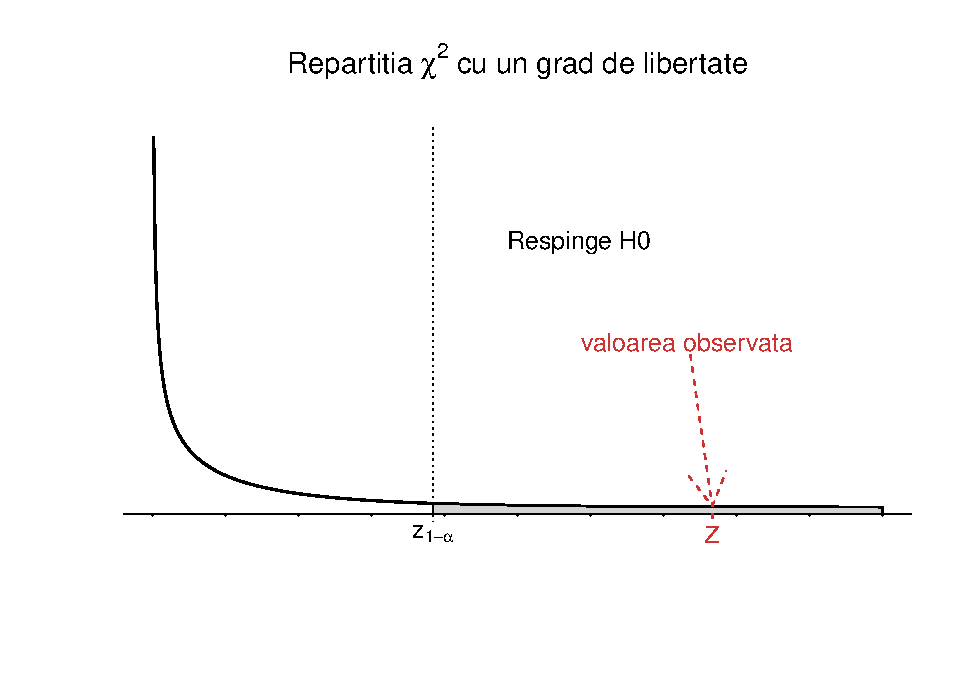
\includegraphics[width=0.8\linewidth]{Lab_5_files/figure-latex/unnamed-chunk-19-1} \end{center}

Același rezultat se obține și dacă folosim testul \texttt{prop.test},
acesta fiind un caz particular al testului hi-pătrat:

\begin{Shaded}
\begin{Highlighting}[]
\KeywordTok{prop.test}\NormalTok{(Mobs)}

    \DecValTok{2}\OperatorTok{-}\NormalTok{sample test }\ControlFlowTok{for}\NormalTok{ equality of proportions with continuity}
\NormalTok{    correction}

\NormalTok{data}\OperatorTok{:}\StringTok{  }\NormalTok{Mobs}
\NormalTok{X}\OperatorTok{-}\NormalTok{squared =}\StringTok{ }\FloatTok{7.6665}\NormalTok{, df =}\StringTok{ }\DecValTok{1}\NormalTok{, p}\OperatorTok{-}\NormalTok{value =}\StringTok{ }\FloatTok{0.005626}
\NormalTok{alternative hypothesis}\OperatorTok{:}\StringTok{ }\NormalTok{two.sided}
\DecValTok{95}\NormalTok{ percent confidence interval}\OperatorTok{:}
\StringTok{ }\FloatTok{0.0002463116} \FloatTok{0.0035536884}
\NormalTok{sample estimates}\OperatorTok{:}
\NormalTok{prop }\DecValTok{1}\NormalTok{ prop }\DecValTok{2} 
\FloatTok{0.0026} \FloatTok{0.0007} 
\end{Highlighting}
\end{Shaded}

\subsection{Metoda testului bazat pe raportul de
verosimilități}\label{metoda-testului-bazat-pe-raportul-de-verosimilitati}

În contextul exemplului de mai sus vrem să vedem testul bazat pe
raportul de verosimilitate. Considerând modelul multinomial
\((n_{11},n_{12},n_{21},n_{22})\sim \mathcal{M}(n;p_{11},p_{12},p_{21},p_{22})\),
obținem raportul de verosimilitate

\[
  \Lambda(x)=\frac{\sup_{\theta\in\Theta_0}L(\theta|x)}{\sup_{\theta\in\Theta}L(\theta|x)}=\prod_{i=1}^{2}\prod_{j=1}^{2}\left(\frac{n_{i\cdot}\times n_{\cdot j}}{n\times n_{ij}}\right)^{n_{ij}}
\]

și din teorema lui Wilks (cazul multidimensional) avem
\(-2\log\Lambda\to\chi^2(d-d_0)\) unde \(d=\dim(\Theta)\) și
\(d_0=\dim(\Theta_0)\). În cazul nostru

\[
  \begin{array}{ll}
    \Theta = \left\{(p_{11},p_{12},p_{21},p_{22})\,|\,p_{ij}\in(0,1),\,\sum_{i=1}^{2}\sum_{j=1}^{2}p_{ij}=1\right\}\\
    \Theta_0 = \left\{(p_{1}q_1,p_{1}q_2,p_{2}q_1,p_{2}q_2)\,|\,p_{i},q_j\in(0,1),\,\sum_{i=1}^{2}p_{i}=1,\,\sum_{j=1}^{2}q_j=1\right\}
  \end{array}
\]

unde \(p_i\) și \(q_j\) sunt repartițiile marginale. Obținem că
\(\dim(\Theta)=4-1\) iar \(\dim(\Theta_0)=4-2\), deci
\(-2\log\Lambda\to\chi^2(1)\).

\begin{Shaded}
\begin{Highlighting}[]
\CommentTok{# Observat}
\NormalTok{n11 =}\StringTok{ }\DecValTok{13}
\NormalTok{n1o =}\StringTok{ }\DecValTok{5000}
\NormalTok{n12 =}\StringTok{ }\NormalTok{n1o}\OperatorTok{-}\NormalTok{n11}

\NormalTok{n21 =}\StringTok{ }\DecValTok{7}
\NormalTok{n2o =}\StringTok{ }\DecValTok{10000}
\NormalTok{n22 =}\StringTok{ }\NormalTok{n2o}\OperatorTok{-}\NormalTok{n21}

\NormalTok{no1 =}\StringTok{ }\NormalTok{n11}\OperatorTok{+}\NormalTok{n21}
\NormalTok{no2 =}\StringTok{ }\NormalTok{n12}\OperatorTok{+}\NormalTok{n22}

\NormalTok{LRT =}\StringTok{ }\NormalTok{n11}\OperatorTok{*}\KeywordTok{log}\NormalTok{((n1o}\OperatorTok{*}\NormalTok{no1)}\OperatorTok{/}\NormalTok{(n}\OperatorTok{*}\NormalTok{n11)) }\OperatorTok{+}\StringTok{ }\NormalTok{n12}\OperatorTok{*}\KeywordTok{log}\NormalTok{((n1o}\OperatorTok{*}\NormalTok{no2)}\OperatorTok{/}\NormalTok{(n}\OperatorTok{*}\NormalTok{n12)) }\OperatorTok{+}\StringTok{ }
\StringTok{  }\NormalTok{n21}\OperatorTok{*}\KeywordTok{log}\NormalTok{((n2o}\OperatorTok{*}\NormalTok{no1)}\OperatorTok{/}\NormalTok{(n}\OperatorTok{*}\NormalTok{n21)) }\OperatorTok{+}\StringTok{ }\NormalTok{n22}\OperatorTok{*}\KeywordTok{log}\NormalTok{((n2o}\OperatorTok{*}\NormalTok{no2)}\OperatorTok{/}\NormalTok{(n}\OperatorTok{*}\NormalTok{n22))}
\NormalTok{LRT =}\StringTok{ }\OperatorTok{-}\DecValTok{2}\OperatorTok{*}\NormalTok{LRT}
\NormalTok{LRT}
\NormalTok{[}\DecValTok{1}\NormalTok{] }\FloatTok{8.354617}

\NormalTok{pval =}\StringTok{ }\DecValTok{1}\OperatorTok{-}\KeywordTok{pchisq}\NormalTok{(LRT,}\DecValTok{1}\NormalTok{) }\CommentTok{#df = 1}
\NormalTok{pval}
\NormalTok{[}\DecValTok{1}\NormalTok{] }\FloatTok{0.003847085}
\end{Highlighting}
\end{Shaded}

\begin{center}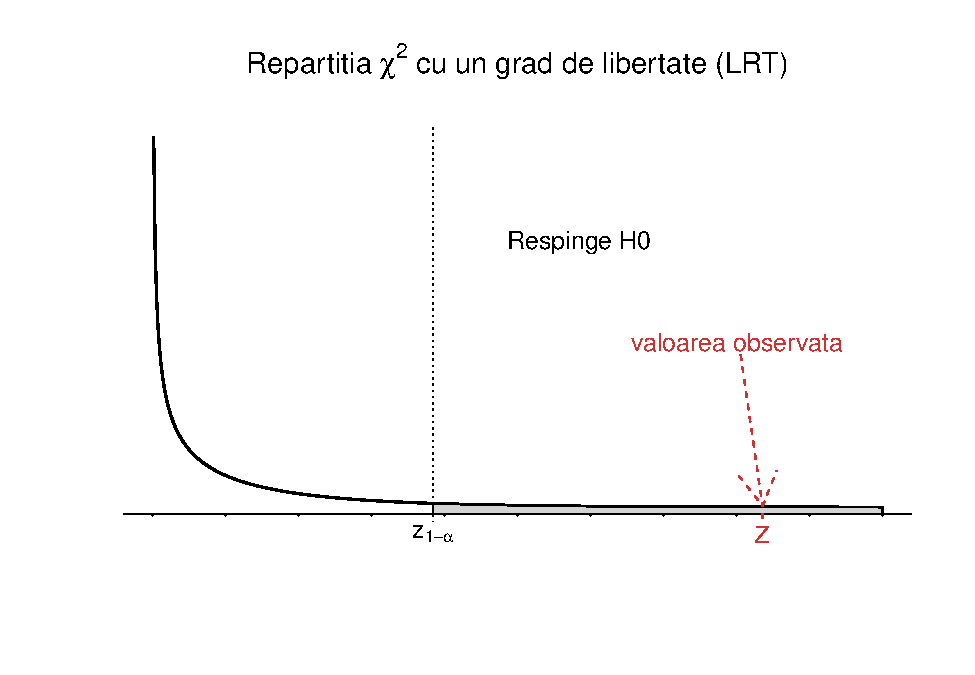
\includegraphics[width=0.8\linewidth]{Lab_5_files/figure-latex/unnamed-chunk-22-1} \end{center}

Să creăm o funcție care automatizează procesul:

\begin{Shaded}
\begin{Highlighting}[]
\NormalTok{LRT1 =}\StringTok{ }\ControlFlowTok{function}\NormalTok{(dat)\{}
  \CommentTok{# dat este sub forma de matrice }
\NormalTok{  rs =}\StringTok{ }\KeywordTok{rowSums}\NormalTok{(dat) }\CommentTok{# apply(dat, 1, sum)}
\NormalTok{  cs =}\StringTok{ }\KeywordTok{colSums}\NormalTok{(dat) }\CommentTok{# apply(dat, 2, sum)}
  
\NormalTok{  n =}\StringTok{ }\KeywordTok{sum}\NormalTok{(dat)}
  
\NormalTok{  expected <-}\StringTok{ }\KeywordTok{outer}\NormalTok{(rs,cs,}\StringTok{"*"}\NormalTok{)}\OperatorTok{/}\NormalTok{n}
  
\NormalTok{  lrt <-}\StringTok{ }\OperatorTok{-}\DecValTok{2}\OperatorTok{*}\KeywordTok{sum}\NormalTok{(dat }\OperatorTok{*}\StringTok{ }\KeywordTok{log}\NormalTok{(expected}\OperatorTok{/}\NormalTok{dat)) }
  
\NormalTok{  dm =}\StringTok{ }\KeywordTok{dim}\NormalTok{(dat) }\CommentTok{# dimensiunea tabloului pentru a calcula gradele de libertate}
\NormalTok{  pval =}\StringTok{ }\DecValTok{1}\OperatorTok{-}\KeywordTok{pchisq}\NormalTok{(lrt,(dm[}\DecValTok{1}\NormalTok{]}\OperatorTok{-}\DecValTok{1}\NormalTok{)}\OperatorTok{*}\NormalTok{(dm[}\DecValTok{2}\NormalTok{]}\OperatorTok{-}\DecValTok{1}\NormalTok{))}
  
  \KeywordTok{cat}\NormalTok{(}\StringTok{"Statistica LRT este "}\NormalTok{, lrt, }\StringTok{"}\CharTok{\textbackslash{}n}\StringTok{"}\NormalTok{)}
  \KeywordTok{cat}\NormalTok{(}\StringTok{"P-valoarea testului bazat pe raportul de verosimilitate este "}\NormalTok{, pval)}
  
  \KeywordTok{return}\NormalTok{(}\KeywordTok{list}\NormalTok{(}\DataTypeTok{statistic =}\NormalTok{ lrt, }\DataTypeTok{pvalue =}\NormalTok{ pval))}
\NormalTok{\}}

\NormalTok{Mobs =}\StringTok{ }\KeywordTok{matrix}\NormalTok{(}\KeywordTok{c}\NormalTok{(n11,n12,n21,n22),}\DataTypeTok{ncol =} \DecValTok{2}\NormalTok{, }\DataTypeTok{byrow =}\NormalTok{ T, }
              \DataTypeTok{dimnames =} \KeywordTok{list}\NormalTok{(}\KeywordTok{c}\NormalTok{(}\StringTok{"OC"}\NormalTok{,}\StringTok{"non-OC"}\NormalTok{), }\KeywordTok{c}\NormalTok{(}\StringTok{"MI"}\NormalTok{, }\StringTok{"non-MI"}\NormalTok{)))}

\KeywordTok{LRT1}\NormalTok{(Mobs) }
\NormalTok{Statistica LRT este  }\FloatTok{8.354617} 
\NormalTok{P}\OperatorTok{-}\NormalTok{valoarea testului bazat pe raportul de verosimilitate este  }\FloatTok{0.003847085}
\OperatorTok{$}\NormalTok{statistic}
\NormalTok{[}\DecValTok{1}\NormalTok{] }\FloatTok{8.354617}

\OperatorTok{$}\NormalTok{pvalue}
\NormalTok{[}\DecValTok{1}\NormalTok{] }\FloatTok{0.003847085}
\end{Highlighting}
\end{Shaded}

\section{Testul exact al lui Fisher}\label{testul-exact-al-lui-fisher}

\begin{rmdexercise}
Să presupunem că vrem să investigăm legătura dintre regimul bogat în
sare și decesul datorat unei boli cardiovasculare (CVD). Să presupunem
că suntem în contextul unui studiu retrospectiv efectuat pe un grup de
bărbați cu vârste cuprinse între 50 și 54 de ani dintr-o anumită regiune
geografică care au decedat pe parcursul unui luni. S-a încercat
introducerea în studiu a unui grup cât mai omogen (s-a încercat
includerea în studiu a unui număr egal de persoane care au decedat din
cauză de CVD și care au decedat din alte cauze).
\end{rmdexercise}

S-a obținut următorul tabel:

\rowcolors{2}{gray!6}{white}

\begin{longtable}{lccccccccc}
\hiderowcolors
\toprule
  & Ridicat Sare & Scazut Sare & Total\\
\midrule
\endfirsthead
\multicolumn{10}{@{}l}{\textit{(continued)}}\\
\toprule
  & Ridicat Sare & Scazut Sare & Total\\
\midrule
\endhead
\
\endfoot
\bottomrule
\endlastfoot
\showrowcolors
non-CVD & 2 & 23 & 25\\
CVD & 5 & 30 & 35\\
Total & 7 & 53 & 60\\*
\end{longtable}

\rowcolors{2}{white}{white}

Tabelul pe care ne așteptam să-l obținem (\(H_0\)) este:

\begin{Shaded}
\begin{Highlighting}[]
\CommentTok{# Observat}
\NormalTok{n11 =}\StringTok{ }\DecValTok{2}
\NormalTok{n1o =}\StringTok{ }\DecValTok{25}
\NormalTok{n12 =}\StringTok{ }\NormalTok{n1o}\OperatorTok{-}\NormalTok{n11}

\NormalTok{n21 =}\StringTok{ }\DecValTok{5}
\NormalTok{n2o =}\StringTok{ }\DecValTok{35}
\NormalTok{n22 =}\StringTok{ }\NormalTok{n2o}\OperatorTok{-}\NormalTok{n21}

\NormalTok{no1 =}\StringTok{ }\NormalTok{n11}\OperatorTok{+}\NormalTok{n21}
\NormalTok{no2 =}\StringTok{ }\NormalTok{n12}\OperatorTok{+}\NormalTok{n22}

\NormalTok{n =}\StringTok{ }\NormalTok{n1o}\OperatorTok{+}\NormalTok{n2o}

\CommentTok{#Asteptat}
\NormalTok{e11 =}\StringTok{ }\NormalTok{n1o}\OperatorTok{*}\NormalTok{no1}\OperatorTok{/}\NormalTok{n}
\NormalTok{e12 =}\StringTok{ }\NormalTok{n1o}\OperatorTok{*}\NormalTok{no2}\OperatorTok{/}\NormalTok{n}
\NormalTok{e21 =}\StringTok{ }\NormalTok{n2o}\OperatorTok{*}\NormalTok{no1}\OperatorTok{/}\NormalTok{n}
\NormalTok{e22 =}\StringTok{ }\NormalTok{n2o}\OperatorTok{*}\NormalTok{no2}\OperatorTok{/}\NormalTok{n}

\NormalTok{MobsF =}\StringTok{ }\KeywordTok{matrix}\NormalTok{(}\KeywordTok{c}\NormalTok{(n11,n12,n21,n22),}\DataTypeTok{ncol =} \DecValTok{2}\NormalTok{, }\DataTypeTok{byrow =}\NormalTok{ T, }
               \DataTypeTok{dimnames =} \KeywordTok{list}\NormalTok{(}\KeywordTok{c}\NormalTok{(}\StringTok{"non-CVD"}\NormalTok{, }\StringTok{"CVD"}\NormalTok{), }
                               \KeywordTok{c}\NormalTok{(}\StringTok{"Ridicat Sare"}\NormalTok{, }\StringTok{"Scazut Sare"}\NormalTok{)))}

\NormalTok{MexpF =}\StringTok{ }\KeywordTok{matrix}\NormalTok{(}\KeywordTok{c}\NormalTok{(e11,e12,e21,e22),}\DataTypeTok{ncol =} \DecValTok{2}\NormalTok{, }\DataTypeTok{byrow =}\NormalTok{ T, }
               \DataTypeTok{dimnames =} \KeywordTok{list}\NormalTok{(}\KeywordTok{c}\NormalTok{(}\StringTok{"non-CVD"}\NormalTok{, }\StringTok{"CVD"}\NormalTok{), }
                               \KeywordTok{c}\NormalTok{(}\StringTok{"Ridicat Sare"}\NormalTok{, }\StringTok{"Scazut Sare"}\NormalTok{)))}
\end{Highlighting}
\end{Shaded}

\rowcolors{2}{gray!6}{white}

\begin{longtable}{lcccccc}
\hiderowcolors
\toprule
  & Ridicat Sare & Scazut Sare\\
\midrule
\endfirsthead
\multicolumn{7}{@{}l}{\textit{(continued)}}\\
\toprule
  & Ridicat Sare & Scazut Sare\\
\midrule
\endhead
\
\endfoot
\bottomrule
\endlastfoot
\showrowcolors
non-CVD & 2.916667 & 22.08333\\
CVD & 4.083333 & 30.91667\\*
\end{longtable}

\rowcolors{2}{white}{white}

Observăm că avem două celule în tabelul așteptat care conțin mai puțin
de 5 observații prin urmare nu putem folosi metodele de mai sus
(aproximarea normală, testul lui Pearson sau testul bazat pe raportul de
verosimilitate). Dacă am încerca am obține:

\begin{Shaded}
\begin{Highlighting}[]
\CommentTok{# Testul lui Pearson (Hi patrat)}

\KeywordTok{chisq.test}\NormalTok{(MobsF)}

\NormalTok{    Pearson}\StringTok{'s Chi-squared test with Yates'}\NormalTok{ continuity correction}

\NormalTok{data}\OperatorTok{:}\StringTok{  }\NormalTok{MobsF}
\NormalTok{X}\OperatorTok{-}\NormalTok{squared =}\StringTok{ }\FloatTok{0.11552}\NormalTok{, df =}\StringTok{ }\DecValTok{1}\NormalTok{, p}\OperatorTok{-}\NormalTok{value =}\StringTok{ }\FloatTok{0.7339}

\CommentTok{# Testul bazat pe raportul de verosimilitate}

\KeywordTok{LRT1}\NormalTok{(MobsF)}
\NormalTok{Statistica LRT este  }\FloatTok{0.5810517} 
\NormalTok{P}\OperatorTok{-}\NormalTok{valoarea testului bazat pe raportul de verosimilitate este  }\FloatTok{0.4459004}
\OperatorTok{$}\NormalTok{statistic}
\NormalTok{[}\DecValTok{1}\NormalTok{] }\FloatTok{0.5810517}

\OperatorTok{$}\NormalTok{pvalue}
\NormalTok{[}\DecValTok{1}\NormalTok{] }\FloatTok{0.4459004}
\end{Highlighting}
\end{Shaded}

Enumerăm tabelele și probabilitățile lor de apariție:

\begin{Shaded}
\begin{Highlighting}[]
\CommentTok{# Fixez marginalele}

\NormalTok{n1o =}\StringTok{ }\DecValTok{25}
\NormalTok{n2o =}\StringTok{ }\DecValTok{35}
  
\NormalTok{no1 =}\StringTok{ }\DecValTok{7}
\NormalTok{no2 =}\StringTok{ }\DecValTok{53}

\ControlFlowTok{for}\NormalTok{ (i }\ControlFlowTok{in} \DecValTok{0}\OperatorTok{:}\DecValTok{7}\NormalTok{)\{}
  \KeywordTok{cat}\NormalTok{(}\StringTok{"-------------------------------------}\CharTok{\textbackslash{}n}\StringTok{"}\NormalTok{)}
  \KeywordTok{cat}\NormalTok{(}\StringTok{"Tabelul "}\NormalTok{, i}\OperatorTok{+}\DecValTok{1}\NormalTok{, }\StringTok{" :}\CharTok{\textbackslash{}n}\StringTok{"}\NormalTok{)}
  
  \CommentTok{# calculez valorile din tabel}
\NormalTok{  n11 =}\StringTok{ }\NormalTok{i}
\NormalTok{  n12 =}\StringTok{ }\NormalTok{n1o }\OperatorTok{-}\StringTok{ }\NormalTok{n11}
\NormalTok{  n21 =}\StringTok{ }\NormalTok{no1 }\OperatorTok{-}\StringTok{ }\NormalTok{n11}
\NormalTok{  n22 =}\StringTok{ }\NormalTok{no2 }\OperatorTok{-}\StringTok{ }\NormalTok{n12}
  
\NormalTok{  MobsF1 =}\StringTok{ }\KeywordTok{matrix}\NormalTok{(}\KeywordTok{c}\NormalTok{(n11,n12,n21,n22),}\DataTypeTok{ncol =} \DecValTok{2}\NormalTok{, }\DataTypeTok{byrow =}\NormalTok{ T, }
                  \DataTypeTok{dimnames =} \KeywordTok{list}\NormalTok{(}\KeywordTok{c}\NormalTok{(}\StringTok{"non-CVD"}\NormalTok{, }\StringTok{"CVD"}\NormalTok{), }
                                  \KeywordTok{c}\NormalTok{(}\StringTok{"Ridicat Sare"}\NormalTok{, }\StringTok{"Scazut Sare"}\NormalTok{)))}
  
  \KeywordTok{print}\NormalTok{(MobsF1)}
  
  \KeywordTok{cat}\NormalTok{(}\StringTok{"Probabilitatea de a obtine tabelul "}\NormalTok{, i}\OperatorTok{+}\DecValTok{1}\NormalTok{, }\StringTok{" este "}\NormalTok{, }
      \KeywordTok{dhyper}\NormalTok{(i, no1, no2, n1o), }\StringTok{"}\CharTok{\textbackslash{}n}\StringTok{"}\NormalTok{)}
  \KeywordTok{cat}\NormalTok{(}\StringTok{"-------------------------------------}\CharTok{\textbackslash{}n}\StringTok{"}\NormalTok{)}
\NormalTok{\}}
\OperatorTok{-------------------------------------}
\NormalTok{Tabelul  }\DecValTok{1}  \OperatorTok{:}
\StringTok{        }\NormalTok{Ridicat Sare Scazut Sare}
\NormalTok{non}\OperatorTok{-}\NormalTok{CVD            }\DecValTok{0}          \DecValTok{25}
\NormalTok{CVD                }\DecValTok{7}          \DecValTok{28}
\NormalTok{Probabilitatea de a obtine tabelul  }\DecValTok{1}\NormalTok{  este  }\FloatTok{0.0174117} 
\OperatorTok{-------------------------------------}
\OperatorTok{-------------------------------------}
\NormalTok{Tabelul  }\DecValTok{2}  \OperatorTok{:}
\StringTok{        }\NormalTok{Ridicat Sare Scazut Sare}
\NormalTok{non}\OperatorTok{-}\NormalTok{CVD            }\DecValTok{1}          \DecValTok{24}
\NormalTok{CVD                }\DecValTok{6}          \DecValTok{29}
\NormalTok{Probabilitatea de a obtine tabelul  }\DecValTok{2}\NormalTok{  este  }\FloatTok{0.1050706} 
\OperatorTok{-------------------------------------}
\OperatorTok{-------------------------------------}
\NormalTok{Tabelul  }\DecValTok{3}  \OperatorTok{:}
\StringTok{        }\NormalTok{Ridicat Sare Scazut Sare}
\NormalTok{non}\OperatorTok{-}\NormalTok{CVD            }\DecValTok{2}          \DecValTok{23}
\NormalTok{CVD                }\DecValTok{5}          \DecValTok{30}
\NormalTok{Probabilitatea de a obtine tabelul  }\DecValTok{3}\NormalTok{  este  }\FloatTok{0.2521695} 
\OperatorTok{-------------------------------------}
\OperatorTok{-------------------------------------}
\NormalTok{Tabelul  }\DecValTok{4}  \OperatorTok{:}
\StringTok{        }\NormalTok{Ridicat Sare Scazut Sare}
\NormalTok{non}\OperatorTok{-}\NormalTok{CVD            }\DecValTok{3}          \DecValTok{22}
\NormalTok{CVD                }\DecValTok{4}          \DecValTok{31}
\NormalTok{Probabilitatea de a obtine tabelul  }\DecValTok{4}\NormalTok{  este  }\FloatTok{0.3118225} 
\OperatorTok{-------------------------------------}
\OperatorTok{-------------------------------------}
\NormalTok{Tabelul  }\DecValTok{5}  \OperatorTok{:}
\StringTok{        }\NormalTok{Ridicat Sare Scazut Sare}
\NormalTok{non}\OperatorTok{-}\NormalTok{CVD            }\DecValTok{4}          \DecValTok{21}
\NormalTok{CVD                }\DecValTok{3}          \DecValTok{32}
\NormalTok{Probabilitatea de a obtine tabelul  }\DecValTok{5}\NormalTok{  este  }\FloatTok{0.214378} 
\OperatorTok{-------------------------------------}
\OperatorTok{-------------------------------------}
\NormalTok{Tabelul  }\DecValTok{6}  \OperatorTok{:}
\StringTok{        }\NormalTok{Ridicat Sare Scazut Sare}
\NormalTok{non}\OperatorTok{-}\NormalTok{CVD            }\DecValTok{5}          \DecValTok{20}
\NormalTok{CVD                }\DecValTok{2}          \DecValTok{33}
\NormalTok{Probabilitatea de a obtine tabelul  }\DecValTok{6}\NormalTok{  este  }\FloatTok{0.0818534} 
\OperatorTok{-------------------------------------}
\OperatorTok{-------------------------------------}
\NormalTok{Tabelul  }\DecValTok{7}  \OperatorTok{:}
\StringTok{        }\NormalTok{Ridicat Sare Scazut Sare}
\NormalTok{non}\OperatorTok{-}\NormalTok{CVD            }\DecValTok{6}          \DecValTok{19}
\NormalTok{CVD                }\DecValTok{1}          \DecValTok{34}
\NormalTok{Probabilitatea de a obtine tabelul  }\DecValTok{7}\NormalTok{  este  }\FloatTok{0.01604969} 
\OperatorTok{-------------------------------------}
\OperatorTok{-------------------------------------}
\NormalTok{Tabelul  }\DecValTok{8}  \OperatorTok{:}
\StringTok{        }\NormalTok{Ridicat Sare Scazut Sare}
\NormalTok{non}\OperatorTok{-}\NormalTok{CVD            }\DecValTok{7}          \DecValTok{18}
\NormalTok{CVD                }\DecValTok{0}          \DecValTok{35}
\NormalTok{Probabilitatea de a obtine tabelul  }\DecValTok{8}\NormalTok{  este  }\FloatTok{0.00124467} 
\OperatorTok{-------------------------------------}
\end{Highlighting}
\end{Shaded}

Aplicăm testul exact al lui Fisher \texttt{fisher.test}:

\begin{Shaded}
\begin{Highlighting}[]
\KeywordTok{fisher.test}\NormalTok{(MobsF)}

\NormalTok{    Fisher}\StringTok{'s Exact Test for Count Data}

\StringTok{data:  MobsF}
\StringTok{p-value = 0.6882}
\StringTok{alternative hypothesis: true odds ratio is not equal to 1}
\StringTok{95 percent confidence interval:}
\StringTok{ 0.04625243 3.58478157}
\StringTok{sample estimates:}
\StringTok{odds ratio }
\StringTok{  0.527113 }
\end{Highlighting}
\end{Shaded}

P-valoarea în \texttt{R} este calculată după formula:

\[
  p_{value} = \sum_{\{i:\mathbb{P}(i)\leq \mathbb{P}(obs)\}}\mathbb{P}(i)
\] care în cazul nostru devine

\begin{Shaded}
\begin{Highlighting}[]
\NormalTok{n1o =}\StringTok{ }\DecValTok{25}
\NormalTok{n2o =}\StringTok{ }\DecValTok{35}
  
\NormalTok{no1 =}\StringTok{ }\DecValTok{7}
\NormalTok{no2 =}\StringTok{ }\DecValTok{53}

\NormalTok{n11 =}\StringTok{ }\DecValTok{2}
  
\NormalTok{ps =}\StringTok{ }\KeywordTok{dhyper}\NormalTok{(}\DecValTok{0}\OperatorTok{:}\NormalTok{no1, no1, no2, n1o)}
\NormalTok{pobs =}\StringTok{ }\KeywordTok{dhyper}\NormalTok{(n11, no1, no2, n1o)}

\NormalTok{pval =}\StringTok{ }\KeywordTok{sum}\NormalTok{(ps[ps}\OperatorTok{<=}\NormalTok{pobs])}
\NormalTok{pval}
\NormalTok{[}\DecValTok{1}\NormalTok{] }\FloatTok{0.6881775}
\end{Highlighting}
\end{Shaded}

\section{Date pereche - Testul lui
McNemar}\label{date-pereche---testul-lui-mcnemar}

\begin{rmdexercise}
Ne propunem să comparăm două regimuri de chimioterapie pentru pacienții
cu cancer la sân care au efectuat operația de mastectomie. Cele două
grupuri de tratament investigate ar trebui să fie cât mai comparabile
din punct de vedere al celorlalți factori. Presupunem că un studiu de
potrivire (matched study) a fost pregătit așa încât din fiecare pereche
(potrivită din punct de vedere al vârstei și a condițiilor clinice) s-a
selectat aleator un membru căruia i-a fost administrat tratamentul A iar
celuilalt membru tratamentul B. Pacienții au fost urmăriți pe o perioadă
de 5 ani, iar variabila de interes a fost supraviețuirea în această
perioadă.
\end{rmdexercise}

S-au obținut următoarele date:

\rowcolors{2}{gray!6}{white}

\begin{longtable}{lccccccccc}
\hiderowcolors
\toprule
  & Supravietuit & Decedat & Total\\
\midrule
\endfirsthead
\multicolumn{10}{@{}l}{\textit{(continued)}}\\
\toprule
  & Supravietuit & Decedat & Total\\
\midrule
\endhead
\
\endfoot
\bottomrule
\endlastfoot
\showrowcolors
A & 526 & 95 & 621\\
B & 515 & 106 & 621\\
Total & 1041 & 201 & 1242\\*
\end{longtable}

\rowcolors{2}{white}{white}

Observăm că nu putem folosi testul lui Pearson (cu corecția lui Yates)
deoarece datele nu sunt \emph{independente}. Dacă am folosi am obține:

\begin{Shaded}
\begin{Highlighting}[]
\NormalTok{M1csq =}\StringTok{ }\KeywordTok{matrix}\NormalTok{(}\KeywordTok{c}\NormalTok{(}\DecValTok{526}\NormalTok{,}\DecValTok{95}\NormalTok{,}\DecValTok{515}\NormalTok{,}\DecValTok{106}\NormalTok{),}\DataTypeTok{ncol =} \DecValTok{2}\NormalTok{, }\DataTypeTok{byrow =}\NormalTok{ T)}
\KeywordTok{chisq.test}\NormalTok{(M1csq)}

\NormalTok{    Pearson}\StringTok{'s Chi-squared test with Yates'}\NormalTok{ continuity correction}

\NormalTok{data}\OperatorTok{:}\StringTok{  }\NormalTok{M1csq}
\NormalTok{X}\OperatorTok{-}\NormalTok{squared =}\StringTok{ }\FloatTok{0.59357}\NormalTok{, df =}\StringTok{ }\DecValTok{1}\NormalTok{, p}\OperatorTok{-}\NormalTok{value =}\StringTok{ }\FloatTok{0.441}
\end{Highlighting}
\end{Shaded}

Construim următorul tabel, în care unitatea de analiză nu mai este
\emph{pacientul} ci \emph{perechea} iar perechile sunt clasificate după
cum membrii acelei perechi au supraviețuit sau nu o perioadă
post-operatorie de 5 ani (liniile tabelului sunt rezultatele pacientului
care a urmat tratamentul A iar coloanele sunt rezultatele pacientului
care a urmat tratamentul B):

\rowcolors{2}{gray!6}{white}

\begin{longtable}{lccccccccc}
\hiderowcolors
\toprule
  & Supravietuit & Decedat & Total\\
\midrule
\endfirsthead
\multicolumn{10}{@{}l}{\textit{(continued)}}\\
\toprule
  & Supravietuit & Decedat & Total\\
\midrule
\endhead
\
\endfoot
\bottomrule
\endlastfoot
\showrowcolors
Supravietuit & 510 & 16 & 526\\
Decedat & 5 & 90 & 95\\
Total & 515 & 106 & 621\\*
\end{longtable}

\rowcolors{2}{white}{white}

Observăm că 600 (510+90) de perechi au avut același rezultat (perechi
concordante) și doar 21 de perechi au avut rezultate diferite (perechi
neconcordante).

Aplicăm testul lui McNemar \texttt{mcnemar.test} :

\begin{Shaded}
\begin{Highlighting}[]
\NormalTok{M1 =}\StringTok{ }\KeywordTok{matrix}\NormalTok{(}\KeywordTok{c}\NormalTok{(}\DecValTok{510}\NormalTok{,}\DecValTok{16}\NormalTok{,}\DecValTok{5}\NormalTok{,}\DecValTok{90}\NormalTok{),}\DataTypeTok{ncol =} \DecValTok{2}\NormalTok{, }\DataTypeTok{byrow =}\NormalTok{ T, }
           \DataTypeTok{dimnames =} \KeywordTok{list}\NormalTok{(}\KeywordTok{c}\NormalTok{(}\StringTok{"Supravietuit"}\NormalTok{, }\StringTok{"Decedat"}\NormalTok{), }
                           \KeywordTok{c}\NormalTok{(}\StringTok{"Supravietuit"}\NormalTok{, }\StringTok{"Decedat"}\NormalTok{)))}
\KeywordTok{mcnemar.test}\NormalTok{(M1)}

\NormalTok{    McNemar}\StringTok{'s Chi-squared test with continuity correction}

\StringTok{data:  M1}
\StringTok{McNemar'}\NormalTok{s chi}\OperatorTok{-}\NormalTok{squared =}\StringTok{ }\FloatTok{4.7619}\NormalTok{, df =}\StringTok{ }\DecValTok{1}\NormalTok{, p}\OperatorTok{-}\NormalTok{value =}\StringTok{ }\FloatTok{0.0291}
\end{Highlighting}
\end{Shaded}

\section{\texorpdfstring{Testul \(\chi^2\) de
concordanță}{Testul \textbackslash{}chi\^{}2 de concordanță}}\label{testul-chi2-de-concordanta}

Vom începe prin construirea unui test statistic pentru testarea
parametrilor unei repartiții multinomiale și apoi vom aplica rezultatele
pentru testarea unei ipoteze de concordanță
(\emph{goodness-of-fit})\footnote{A se vedea și testul
  Kolmogorov-Smirnov din
  \href{https://alexamarioarei.github.io/Teaching/2017-2018/Biostat\%20web\%20page/labs/Lab_4.pdf}{Laboratorul
  4}}.

\subsection{Test pentru parametrii unei repartiții
multinomiale}\label{test-pentru-parametrii-unei-repartitii-multinomiale}

Presupunem că \(Y\) este o variabilă aleatoare care ia valori în
mulțimea \(\{y_1,y_2,\ldots,y_c\}\) iar repartiția ei este dată de

\[
\mathbb{P}\circ Y^{-1} = \sum_{j = 1}^{c}p_j\delta_{y_j},
\]

unde \(\mathbb{P}(Y = y_j) = p_{j},\, j\in\{1,2,\ldots,c\}\).

Fie \(Y_1, Y_2,\ldots, Y_n\) un eșantion de talie \(n\) din populația
\(\mathbb{P}\circ Y^{-1}\) și

\[
  N_i = \sum_{k = 1}^{n}\mathbf{1}_{y_i}(Y_k)
\]

numărul de observații care categoria \(y_i\). Observăm că variabilele
aleatoare \(N_1, N_2, \ldots, N_c\) verifică

\[
  N_1 + N_2 +\cdots+ N_c = n.
\]

Putem modela o observație \(Y_k\) dintr-o variabilă discretă cu \(c\)
categorii cu ajutorul unui vector elemente de \(\{0,1\}\),
\((X_1^{(k)}, X_2^{(k)}, \ldots, X_c^{(k)})\), pentru care componenta
\(j\) ia valoarea \(1\) dacă \(Y_k = y_j\) și \(0\) altfel. Funcția de
masă a \(c\)-uplului este

\[
\mathbb{P}((X_1^{(k)}, X_2^{(k)}, \ldots, X_c^{(k)}) = (x_1,x_2,\ldots,x_c)) = p_1^{x_1}p_2^{x_2}\cdots p_c^{x_c}
\] unde \(x_j\in\{0,1\}\) cu \(\sum_{j = 1}^{c}x_j = 1\). Pentru un
eșantion de talie \(n\),
\(\{(X_1^{(k)}, X_2^{(k)}, \ldots, X_c^{(k)}),\, k = 1,2,\ldots, n\}\)
avem

\[
\mathbb{P}\left((X_1^{(k)}, X_2^{(k)}, \ldots, X_c^{(k)}) = (x_1^{(k)},x_2^{(k)},\ldots,x_c^{(k)}), \,k = 1,2,\ldots,n\right) = \prod_{k=1}^{n}p_1^{x_1^{(k)}}p_2^{x_2^{(k)}}\cdots p_c^{x_c^{(k)}} = p_1^{n_1}p_2^{n_2}\cdots p_c^{n_c}
\]

unde \(n_j\) reprezintă numărul de observații din categoria \(y_j\) iar
\(\sum_{j = 1}^{c}n_j = n\).

În următorul exercițiu ne propunem să aplicăm testul bazat pe raportul
de verosimilități pentru efectuarea unui test asupra parametrilor unei
repartiții multinomiale.

\begin{rmdexercise}
Spunem că vectorul \((N_1, N_2,\ldots, N_c)\) este repartizat
multinomial \(\mathcal{M}(n;p_1,p_2,\ldots,p_c)\) dacă

\[
  \mathbb{P}(N_1 = n_1, N_2 = n_2, \ldots, N_c = n_c) = \frac{n!}{n_1!n_2!\cdots n_c!}p_1^{n_1}p_2^{n_2}\cdots p_c^{n_c}
\]

unde \(n_1 + n_2 +\cdots+n_c = n\).

Determinați repartiția marginală a lui \(N_i\).
\end{rmdexercise}

Observăm că

\scriptsize

\begin{align*}
  \mathbb{P}(N_i = n_i) &= \sum_{n_1}\cdots\sum_{n_{i-1}}\sum_{n_{i+1}}\cdots\sum_{n_{c}}\mathbb{P}(N_1 = n_1, \ldots, N_{i-1} = n_{i-1}, N_i = n_i, N_{i+1} = n_{i+1}, \ldots, N_c = n_c),  \; n_1 + \cdots + n_c = n - n_i\\
    &= \sum_{n_1}\cdots\sum_{n_{i-1}}\sum_{n_{i+1}}\cdots\sum_{n_{c}}\frac{n!}{n_1!\cdots n_c!}p_1^{n_1}\cdots p_{c}^{n_c},  \; n_1 + \cdots + n_c = n - n_i\\
    &= \frac{n!p_i^{n_i}}{n_i!(n-n_i)!}\sum_{n_1}\cdots\sum_{n_{i-1}}\sum_{n_{i+1}}\cdots\sum_{n_{c}}\frac{(n-n_i)!}{n_1!\cdots n_{i-1}!n_{i+1}!\cdots n_c!}p_1^{n_1}\cdots p_{i-1}^{n_{i-1}}p_{i+1}^{n_{i+1}}\cdots p_{c}^{n_c},  \; n_1 + \cdots + n_c = n - n_i\\
    &= \binom{n}{n_i}p_i^{n_i}(1-p_i)^{n-n_i}\underbrace{\sum_{n_1}\cdots\sum_{n_{i-1}}\sum_{n_{i+1}}\cdots\sum_{n_{c}}\binom{n-n_i}{n_1,\ldots,n_c}\left(\frac{p_1}{1-p_i}\right)^{n_1}\cdots \left(\frac{p_{i-1}}{1-p_i}\right)^{n_{i-1}}\left(\frac{p_{i+1}}{1-p_i}\right)^{n_{i+1}}\cdots \left(\frac{p_c}{1-p_i}\right)^{n_c}}_{=1}\\
    &= \binom{n}{n_i}p_i^{n_i}(1-p_i)^{n-n_i}
\end{align*}

\normalsize

prin urmare \(N\sim\mathcal{B}(n, p_i)\).

\begin{rmdexercise}
Considerăm ipotezele

\begin{align*}
  H_0: & \{(p_1,p_2,\ldots, p_c) = (\pi_1,\pi_2,\ldots, \pi_c)\}\\
  H_1: & \{\exists i \text{ astfel incat } p_i\neq \pi_i\}
\end{align*}

unde \((\pi_1,\pi_2,\ldots, \pi_c)\) sunt probabilități specificate în
avans. Construiți testul bazat pe raportul de verosimilități
corespunzător.
\end{rmdexercise}

Testul bazat pe raportul de verosimilitate este

\[
  \Lambda(\mathbf{x})=\frac{\sup_{\theta\in\Theta_0}L(\theta|\mathbf{x})}{\sup_{\theta\in\Theta}L(\theta|\mathbf{x})},
\]

unde \(\Theta\) este spațiul parametrilor modelului, \(\Theta_0\) este
spațiul parametrilor corespunzător ipotezei nule iar
\(L(\theta|\mathbf{x})\) este funcția de verosimilitate.

Observăm că spațiul parametrilor corespunzător modelului este

\[
\Theta = \left\{p_1, p_2, \ldots, p_c\,|\,p_{j}\in(0,1),\,\sum_{j = 1}^{c}p_{j} = 1\right\},
\]

cu \(\dim{\Theta} = c-1\), cel corespunzător ipotezei nule este

\[
\Theta_0 = \left\{(p_1,p_2,\ldots, p_c) = (\pi_1,\pi_2,\ldots, \pi_c)\right\}
\]

cu \(\dim{\Theta_0} = 0\) iar funcția de verosimilitate este

\[
  L(p_{j},\,j = 1,\ldots,c\,;\,\mathbf{x}) = \mathbb{P}(N_{j} = n_{j}, \,j = 1,\ldots,c) = \frac{n!}{\prod_{j = 1}^{c} n_{j}!}\prod_{j = 1}^{c} p_{j}^{n_{j}}.
\]

Observăm că

\[
  \sup_{\theta\in\Theta_0}L(\theta|\mathbf{x}) = \mathbb{P}_{H_0}(N_1 = n_1, N_2 = n_2, \ldots, N_c = n_c) = \frac{n!}{\prod_{j = 1}^{c} n_{j}!}\prod_{j = 1}^{c} \pi_{j}^{n_{j}}.
\]

Pentru a determina estimatorul de verosimilitate maximă pe \(\Theta\)
trebuie să rezolvăm problema de optimizare:

\[
  \left\{\begin{array}{ll}
    \max_{\theta\in\Theta} \log L(\theta|\mathbf{x}) = \max \log{\left(\frac{n!}{\prod_{j = 1}^{c} n_{j}!}\prod_{j = 1}^{c} p_{j}^{n_{j}}\right)}\\
    \sum_{j = 1}^{c}p_{j} = 1
  \end{array}\right.
\]

Cum logaritmul funcției de verosimilitate este

\[
\log{\left(\frac{n!}{\prod_{j = 1}^{c} n_{j}!}\prod_{j = 1}^{c} p_{j}^{n_{j}}\right)} = \log\left(\frac{n!}{\prod_{j = 1}^{c} n_{j}!}\right) + \sum_{j = 1}^{c}n_{j}\log{p_j}
\]

iar \(p_c = 1 - p_1 -\cdots p_{c-1}\), rezolvând ecuația de
verosimilitate \(\frac{\partial\log{L}}{\partial p_j} = 0\) deducem

\[
\left\{\begin{array}{llll}
  \frac{n_1}{p_1} - \frac{n_c}{1 - p_1 - p_2 -\cdots -p_{c-1}} = 0\\
  \frac{n_2}{p_2} - \frac{n_c}{1 - p_1 - p_2 -\cdots -p_{c-1}} = 0\\
  \cdots\cdots\cdots\cdots\cdots\cdots\cdots\cdots\\
  \frac{n_{c-1}}{p_{c-1}} - \frac{n_c}{1 - p_1 - p_2 -\cdots -p_{c-1}} = 0\\
\end{array}\right.
\]

de unde

\[
  \frac{n_1}{p_1} = \frac{n_2}{p_2} = \cdots = \frac{n_c}{p_c} = \frac{\sum_{j = 1}^{c}n_j}{\sum_{j = 1}^{c}p_j} = n,
\]

deci \(\hat{p}_{j} = \frac{n_j}{n}\).

Raportul de verosimilitate devine

\[
\Lambda(\mathbf{x})=\frac{\sup_{\theta\in\Theta_0}L(\theta|\mathbf{x})}{\sup_{\theta\in\Theta}L(\theta|\mathbf{x})} = \frac{\prod_{j = 1}^{c} \pi_{j}^{n_{j}}}{\prod_{j = 1}^{c} \left(\frac{n_{j}}{n}\right)^{n_{j}}} = \prod_{j = 1}^{c}\left(\frac{n\pi_{j}}{n_j}\right)^{n_{j}}
\]

și aplicând
\href{https://en.wikipedia.org/wiki/Likelihood-ratio_test}{Teorema lui
Wilks} găsim

\[
  -2\log \Lambda(\mathbf{x}) = 2\sum_{j = 1}^{c} n_{j}\log\left(\frac{n_{j}}{n\times \pi_{j}}\right) \underset{n\to\infty}{\overset{d}{\longrightarrow}}\chi^2(\underbrace{\dim{\Theta} - \dim{\Theta_0}}_{(c-1)-0}) = \chi^2(c-1).
\]

Prin urmare, regiunea critică a testului asimptotic de nivel \(\alpha\)
bazat pe raportul de verosimilitate este

\[
  C = \left\{\mathbf{x} \,|\, -2\log \Lambda(\mathbf{x}) > \chi^2_{1-\alpha}(c-1)\right\}.
\]

O metodă alternativă este bazată pe statistica \(\chi^2\) a lui Pearson,
\citep{Pearson1900}, care este dată de

\[
  X^2 = \sum_{j = 1}^{c}\frac{(O_{j} - E_{j})^2}{E_{j}}
\]

unde \(O_{j} = n_{j}\) sunt efectivele observate iar \(E_{j}\) sunt
efectivele pe care ne așteptăm să le observăm dacă ipoteza nulă ar fi
adevărată (sub \(H_0\), repartiția condiționată a lui \(N_{j}\) la
\(\sum_{j = 1}^{c}N_{j} = n\) este \(\mathcal{B}(n,p_{j})\)),

\[
  E_{j} = \mathbb{E}_{H_0}[N_{j}] = n \pi_j
\]

ceea ce implică

\[
  X^2 = \sum_{j = 1}^{c}\frac{\left(N_{j} - n \pi_j\right)^2}{n \pi_j}.
\]

Karl Pearson a arătat că această statistică este asimptotic repartizată

\[
  X^2 = \sum_{j = 1}^{c}\frac{\left(N_{j} - n \pi_j\right)^2}{n \pi_j} \underset{n\to\infty}{\overset{d}{\longrightarrow}} \chi^2(c-1)
\]

prin urmare testul \(\chi^2\) a lui Pearson de nivel \(\alpha\), pentru
ipotezele \(H_0\,vs\,H_1\) conduce la aceeași regiune critică ca și
testul bazat pe raportul de verosimilitate. În practică, testul
\(\chi^2\) a lui Pearson se folosește atunci când efectivele observate
verifică \(E_j\geq 5\), \(j = 1,\ldots, c\).

\subsection{Test de concordanță}\label{test-de-concordanta}

Fie \(x_1,X_2,\ldots,X_n\) un eșantion de talie \(n\) dintr-o populație
(necunoscută) \(F\) și ne propunem să testăm ipotezele

\[
  H_0:\, \{F = F_0\}\quad vs\quad H_1:\,\{F\neq F_0\}
\]

unde \(F_0\) este o repartiție fixată sau face parte dintr-o familie de
repartiții \(\{F_0(x;\theta)|\theta\in\Theta\}\). Pentru a aplica testul
\(\chi^2\) pentru parametrii unei repartiții multinomiale trebuie să
partiționăm mulțimea valorilor \(\mathcal{X}\) într-o serie de
subintervale \(I_1, I_2,\ldots,I_c\) astfel ca efectivele pe care ne
așteptăm să le observăm \(E_j = n\pi_j(\theta)\geq 5\), unde ipoteza
nulă \(H_0\) implică \(F_0(I_j;\theta) = \pi_j(\theta)\). O variantă
este să construim intervalele astfel ca ele să aibă aceeași
probabilitate \(\frac{1}{c}\) și să alegem \(c\) pentru care
\(\frac{n}{c}\geq 5\).

Observăm că pentru ipoteza nulă \(H_0:\, \{F = F_0\}\), cu \(F_0\)
fixată, putem folosi testul bazat pe statistica de test \(\chi^2\) a lui
Pearson

\[
  X^2 = \sum_{j = 1}^{c}\frac{\left(N_{j} - n \pi_j\right)^2}{n \pi_j}\underset{n\to\infty}{\overset{d}{\longrightarrow}} \chi^2(c-1)
\] cu \(\pi_j = F_0(I_j)\) iar \(N_j\) sunt efectivele din intervalele
\(I_j\).

În cazul ipotezei nule compuse

\[
H_0:\, \{F = F_0(\theta)|\theta\in\Theta\},
\]

unde presupunem că \(\dim(\Theta) = r\leq c-2\), putem determina
estimatorul de verosimilitate maximă a lui \(\pi_{j}(\theta)\) pe baza
estimatorului de verosimilitate maximă a lui \(\theta\),
\(\bar{\theta}\) (să ne reamintim din proprietatea de invarianță că dacă
\(\bar{\theta}\) este EVM pentru \(\theta\) atunci
\(\pi_{j}(\bar{\theta})\) este EVM pentru \(\pi_{j}(\theta)\)).
Estimatorul \(\bar{\theta}\) maximizează funcția de verosimilitate

\[
L(\theta;x) = \frac{n!}{\prod_{j = 1}^{c} n_{j}!}\prod_{j = 1}^{c} \pi_{j}(\theta)^{n_{j}}
\]

cu restricția \(\sum_{j = 1}^{c} \pi_{j}(\theta)^{n_{j}} = 1\), unde
\(n_1,\ldots, n_c\) sunt efectivele observate în intervalele
\(I_1,\ldots, I_c\). \citep{Cramer1946} a arătat că statistica

\[
  X^2 = \sum_{j = 1}^{c}\frac{\left(N_{j} - n \pi_j(\bar{\theta})\right)^2}{n \pi_j(\bar{\theta})}\underset{n\to\infty}{\overset{d}{\longrightarrow}} \chi^2(c-r-1).
\]

În practică, se folosește de multe ori estimatorul de verosimilitate
maximă \(\hat{\theta}\) a lui \(\theta\) sub modelul \(F_0(\theta)\). Cu
toate acestea, \citep{Lehmann1954} a arătat că repartiția asimptotică a
lui
\(X^2 = \sum_{j = 1}^{c}\frac{\left(N_{j} - n \pi_j(\hat{\theta})\right)^2}{n \pi_j(\hat{\theta})}\)
nu mai este \(\chi^2\) dar este cuprinsă între \(\chi^2(c-r-1)\) și
\(\chi^2(c-1)\).

\begin{rmdexercise}
Un exercițiu constă în extragerea la întâmplare, de către o persoană, a
unei cărți de joc dintr-un pachet amestecat în prealabil, notarea
culorii acesteia (inimă roșie, inimă neagră, romb și treflă) și cărții
în pachet tot aleator. Să presupunem că în urma efectuării exercițiului
pe \(200\) de persoane s-au obținut următoarele rezultate: 35 cărți de
treflă, 51 cărți de romb, 64 cărți de inimă roșie și respectiv 50 cărți
de inimă neagră. Ne propunem să testăm ipotezele

\begin{align*}
  H_0&:\,\{\text{Cele patru culori sunt egal probabile}\}\\
  H_1&:\,\{\text{Cel putin una din cele patru culori este diferita de 0.25}\}
\end{align*}
\end{rmdexercise}

Observăm că dacă notăm cu \(Y\) variabila discretă care ia valori în
mulțimea
\(\{y_1,y_2,y_3,y_4\} = \{\clubsuit, \diamondsuit, \heartsuit, \spadesuit\}\)
și cu \(p_j = \mathbb{P}(Y = y_j)\) atunci ipotezele se scriu

\begin{align*}
  H_0&:\,\{\text{Cele patru culori sunt egal probabile}\} = \{(p_1,p_2,p_3,p_4) = (\pi_1, \pi_2, \pi_3, \pi_4) \,|\, \pi_j = 0.25\}\\
  H_1&:\,\{\text{Cel putin una din cele patru culori este diferita de 0.25}\} = \{\exists j, \text{ astfel ca } p_j\neq 0.25\}
\end{align*}

Avem că tabelul efectivelor observate este

\[
\begin{array}{c|c|c|c}
  \clubsuit & \diamondsuit & \heartsuit & \spadesuit \\
  \hline
  O_1 & O_2 & O_3 & O_4
\end{array} 
=
\begin{array}{c|c|c|c}
  \clubsuit & \diamondsuit & \heartsuit & \spadesuit \\
  \hline
  35 & 51 & 64 & 50
\end{array}
\]

care in R este

\begin{Shaded}
\begin{Highlighting}[]
\NormalTok{tab_observed =}\StringTok{ }\KeywordTok{c}\NormalTok{(}\DecValTok{35}\NormalTok{, }\DecValTok{51}\NormalTok{, }\DecValTok{64}\NormalTok{, }\DecValTok{50}\NormalTok{)}
\end{Highlighting}
\end{Shaded}

iar tabelul efectivelor pe care ne așteptăm să le observăm dacă ipoteza
nulă este adevărată este

\[
\begin{array}{c|c|c|c}
  \clubsuit & \diamondsuit & \heartsuit & \spadesuit \\
  \hline
  E_1 = n\pi_1 & E_2 = n\pi_2 & E_3 = n\pi_3 & E_4 = n\pi_4
\end{array} 
=
\begin{array}{c|c|c|c}
  \clubsuit & \diamondsuit & \heartsuit & \spadesuit \\
  \hline
  50 & 50 & 50 & 50
\end{array}
\]

care în R se scrie

\begin{Shaded}
\begin{Highlighting}[]
\NormalTok{n =}\StringTok{ }\DecValTok{200}
\NormalTok{prob =}\StringTok{ }\KeywordTok{rep}\NormalTok{(}\FloatTok{0.25}\NormalTok{, }\DecValTok{4}\NormalTok{)}

\NormalTok{tab_expected =}\StringTok{ }\NormalTok{n}\OperatorTok{*}\NormalTok{prob}
\end{Highlighting}
\end{Shaded}

Putem calcula acum statistica lui Pearson

\[
  X^2 = \sum_{j = 1}^{c}\frac{(O_{j} - E_{j})^2}{E_{j}} = \sum_{j = 1}^{c}\frac{\left(n_{j} - n \pi_j\right)^2}{n \pi_j}
\]

care devine

\begin{Shaded}
\begin{Highlighting}[]
\NormalTok{alpha =}\StringTok{ }\FloatTok{0.05}
\NormalTok{X2 =}\StringTok{ }\KeywordTok{sum}\NormalTok{((tab_observed }\OperatorTok{-}\StringTok{ }\NormalTok{tab_expected)}\OperatorTok{^}\DecValTok{2}\OperatorTok{/}\NormalTok{tab_expected)}

\CommentTok{# p - valoarea}
\DecValTok{1} \OperatorTok{-}\StringTok{ }\KeywordTok{pchisq}\NormalTok{(X2, }\DataTypeTok{df =} \DecValTok{3}\NormalTok{)}
\NormalTok{[}\DecValTok{1}\NormalTok{] }\FloatTok{0.03774185}
\end{Highlighting}
\end{Shaded}

Acelați rezultat îl obținem și dacă aplicăm funcția
\texttt{chisq.test()}

\begin{Shaded}
\begin{Highlighting}[]
\KeywordTok{chisq.test}\NormalTok{(tab_observed, }\DataTypeTok{p =}\NormalTok{ prob)}

\NormalTok{    Chi}\OperatorTok{-}\NormalTok{squared test }\ControlFlowTok{for}\NormalTok{ given probabilities}

\NormalTok{data}\OperatorTok{:}\StringTok{  }\NormalTok{tab_observed}
\NormalTok{X}\OperatorTok{-}\NormalTok{squared =}\StringTok{ }\FloatTok{8.44}\NormalTok{, df =}\StringTok{ }\DecValTok{3}\NormalTok{, p}\OperatorTok{-}\NormalTok{value =}\StringTok{ }\FloatTok{0.03774}
\end{Highlighting}
\end{Shaded}

Pentru testul bazat pe raportul de verosimilitate maximă avem

\[
  -2\log \Lambda(\mathbf{x}) = -2\sum_{j = 1}^{c} n_{j}\log\left(\frac{n_{j}}{n\times \pi_{j}}\right)
\]

care devine

\begin{Shaded}
\begin{Highlighting}[]
\NormalTok{LRT =}\StringTok{ }\DecValTok{2}\OperatorTok{*}\KeywordTok{sum}\NormalTok{(tab_observed}\OperatorTok{*}\KeywordTok{log}\NormalTok{(tab_observed}\OperatorTok{/}\NormalTok{tab_expected))}

\CommentTok{# p - valoarea}
\DecValTok{1} \OperatorTok{-}\StringTok{ }\KeywordTok{pchisq}\NormalTok{(LRT, }\DataTypeTok{df =} \DecValTok{3}\NormalTok{)}
\NormalTok{[}\DecValTok{1}\NormalTok{] }\FloatTok{0.03431406}
\end{Highlighting}
\end{Shaded}

Ambele proceduri conduc la respingerea ipotezei nule pentru un prag de
semnificație \(\alpha = 0.05\).

\begin{rmdexercise}
Citomegalovirusul uman (CVM) este o boală care poate pune viața în
pericol pentru oamenii cu un sistem imunitar slăbit. Pentru combaterea
virusului, oamenii de știință au studiat genomul CVM pentru a identifica
modul în care se multiplică acesta, observând că o potențială origine de
replicare este dată de aglomerarea de palindroame de ADN (o secvență de
nucleotide care se citesc invers față de complementul secvenței directe:
GGGCATGCCC). Împărțim secvența ADN în 57 de segmente care nu se
suprapun, fiecare având o lungime de 4000 de perechi de bază (lungimea
de 4000 de perechi de bază a fost aleasă pentru a obține un număr
rezonabil de observații), și determinăm pentru fiecare interval numărul
de palindroame care se află în acest interval (setul de date
\href{dataIn/hcmv.data}{hcmv.data} conține locațiile în care se află
palindroamele). Ne propunem să investigăm dacă numărul de palindroame
este repartizat după o repartiție Poisson.
\end{rmdexercise}

Pentru mai multe detalii despre contextul acestui exercițiu se poate
consulta \citep{Nolan1999}. Începem prin citirea setului de date în care
sunt date locațiile palindroamelor în cele 229354 de perechi de bază

\begin{Shaded}
\begin{Highlighting}[]
\NormalTok{palindromes =}\StringTok{ }\KeywordTok{read.table}\NormalTok{(}\StringTok{"dataIn/hcmv.data"}\NormalTok{, }\DataTypeTok{header =} \OtherTok{TRUE}\NormalTok{)}
\KeywordTok{str}\NormalTok{(palindromes)}
\StringTok{'data.frame'}\OperatorTok{:}\StringTok{   }\DecValTok{296}\NormalTok{ obs. of  }\DecValTok{1}\NormalTok{ variable}\OperatorTok{:}
\StringTok{ }\ErrorTok{$}\StringTok{ }\NormalTok{location}\OperatorTok{:}\StringTok{ }\NormalTok{int  }\DecValTok{177} \DecValTok{1321} \DecValTok{1433} \DecValTok{1477} \DecValTok{3248} \DecValTok{3255} \DecValTok{3286} \DecValTok{7263} \DecValTok{9023} \DecValTok{9084}\NormalTok{ ...}
\end{Highlighting}
\end{Shaded}

Putem observa locația palindroamenlor în secvența ADN în figura
următoare

\begin{center}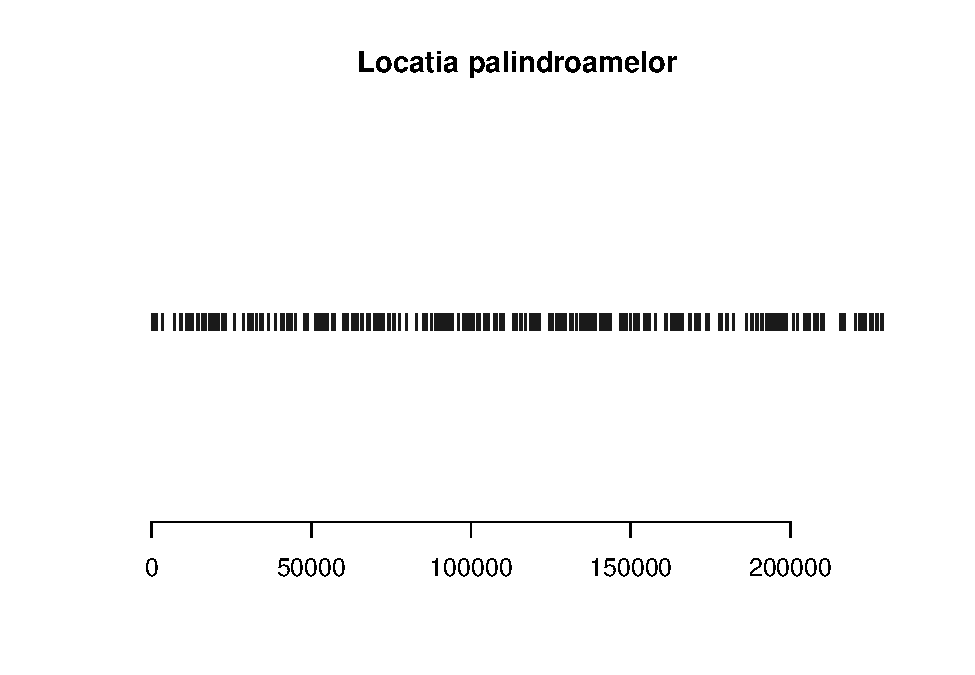
\includegraphics[width=0.8\linewidth]{Lab_5_files/figure-latex/unnamed-chunk-47-1} \end{center}

Ne propunem să ilustrăm cum sunt repartizate efectivele observate pe
intervalele de lungime 4000 perechi de bază:

\begin{Shaded}
\begin{Highlighting}[]
\NormalTok{loc =}\StringTok{ }\NormalTok{palindromes}\OperatorTok{$}\NormalTok{location}

\CommentTok{# capetele intervalelor de lungime 4000}
\NormalTok{intervals =}\StringTok{ }\KeywordTok{seq}\NormalTok{(}\DecValTok{0}\NormalTok{, }\DecValTok{229354}\NormalTok{, }\DataTypeTok{by =} \DecValTok{4000}\NormalTok{)}

\CommentTok{# numarul de intervale}
\NormalTok{n.int =}\StringTok{ }\KeywordTok{length}\NormalTok{(intervals) }\OperatorTok{-}\StringTok{ }\DecValTok{1}

\CommentTok{# calculam efectivele observate}
\NormalTok{count.int =}\StringTok{ }\ControlFlowTok{function}\NormalTok{(i)\{}
  \KeywordTok{sum}\NormalTok{(loc }\OperatorTok{>}\StringTok{ }\NormalTok{intervals[i] }\OperatorTok{&}\StringTok{ }\NormalTok{loc }\OperatorTok{<=}\StringTok{ }\NormalTok{intervals[i}\OperatorTok{+}\DecValTok{1}\NormalTok{])}
\NormalTok{\}}

\NormalTok{counts =}\StringTok{ }\KeywordTok{sapply}\NormalTok{(}\DecValTok{1}\OperatorTok{:}\NormalTok{n.int, count.int)}
\NormalTok{counts}
\NormalTok{ [}\DecValTok{1}\NormalTok{]  }\DecValTok{7}  \DecValTok{1}  \DecValTok{5}  \DecValTok{3}  \DecValTok{8}  \DecValTok{6}  \DecValTok{1}  \DecValTok{4}  \DecValTok{5}  \DecValTok{3}  \DecValTok{6}  \DecValTok{2}  \DecValTok{5}  \DecValTok{8}  \DecValTok{2}  \DecValTok{9}  \DecValTok{6}  \DecValTok{4}  \DecValTok{9}  \DecValTok{4}  \DecValTok{1}  \DecValTok{7}  \DecValTok{7}
\NormalTok{[}\DecValTok{24}\NormalTok{] }\DecValTok{14}  \DecValTok{4}  \DecValTok{4}  \DecValTok{4}  \DecValTok{3}  \DecValTok{5}  \DecValTok{5}  \DecValTok{3}  \DecValTok{6}  \DecValTok{5}  \DecValTok{3}  \DecValTok{9}  \DecValTok{9}  \DecValTok{4}  \DecValTok{5}  \DecValTok{6}  \DecValTok{1}  \DecValTok{7}  \DecValTok{6}  \DecValTok{7}  \DecValTok{5}  \DecValTok{3}  \DecValTok{4}
\NormalTok{[}\DecValTok{47}\NormalTok{]  }\DecValTok{4}  \DecValTok{8} \DecValTok{11}  \DecValTok{5}  \DecValTok{3}  \DecValTok{6}  \DecValTok{3}  \DecValTok{1}  \DecValTok{4}  \DecValTok{8}  \DecValTok{6}
\end{Highlighting}
\end{Shaded}

Observăm că în primul segment ADN de lungime 4000 avem 7 palindroame iar
în al doilea segment avem 1. Repartiția numărului de palindroame este

\begin{center}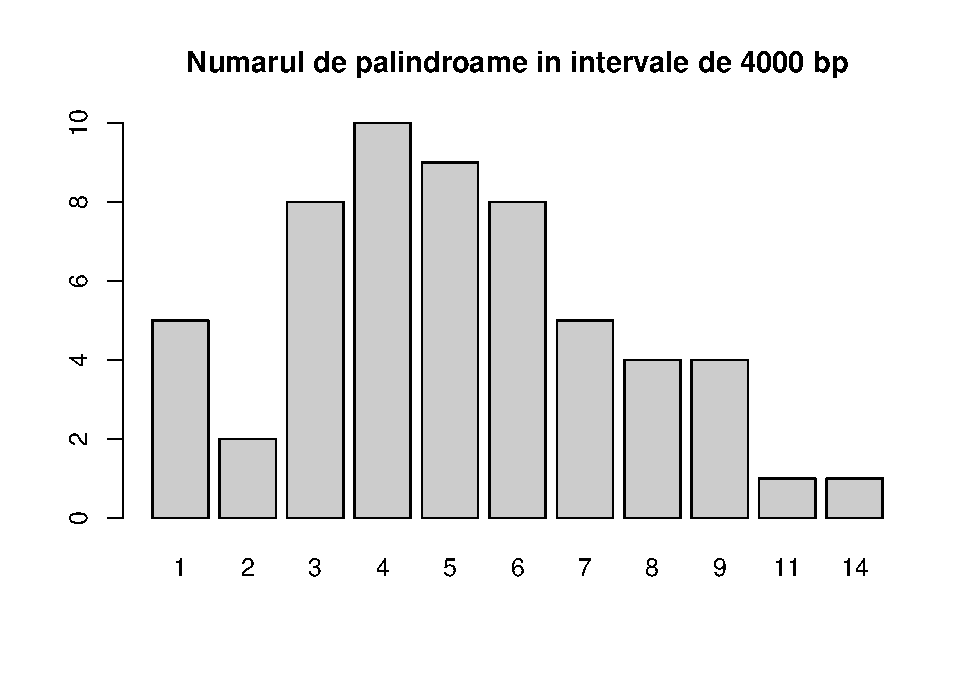
\includegraphics[width=0.8\linewidth]{Lab_5_files/figure-latex/unnamed-chunk-49-1} \end{center}

Din figura de mai sus observăm că din cele 57 de segmente de ADN de 4000
de perechi de bază, 7 conțin cel mult 2 palindroame, 8 conțin 3
palindroame iar 10 conțin 4 palindroame. De asemenea 6 conțin cel puțin
9 palindroame. Aceste segmente acoperă primele 228000 perechi de bază,
ultimele 1354 fiind excluse din construcția intervalelor (acestea mai
conțin 2 palindroame). Prin urmare considerăm doar 294 palindroame.

Estimatorul de verosimilitate maximă pentru parametrul \(\lambda\) a
repartiției Poisson este \(\hat{\lambda} = \bar{X}_n\) și putem să-l
calculăm plecând de la numărul de palindroame pe intervalele de lungime
4000 de perechi de bază:

\begin{Shaded}
\begin{Highlighting}[]
\NormalTok{lambda =}\StringTok{ }\KeywordTok{mean}\NormalTok{(counts)}
\NormalTok{lambda}
\NormalTok{[}\DecValTok{1}\NormalTok{] }\FloatTok{5.157895}
\end{Highlighting}
\end{Shaded}

\begin{center}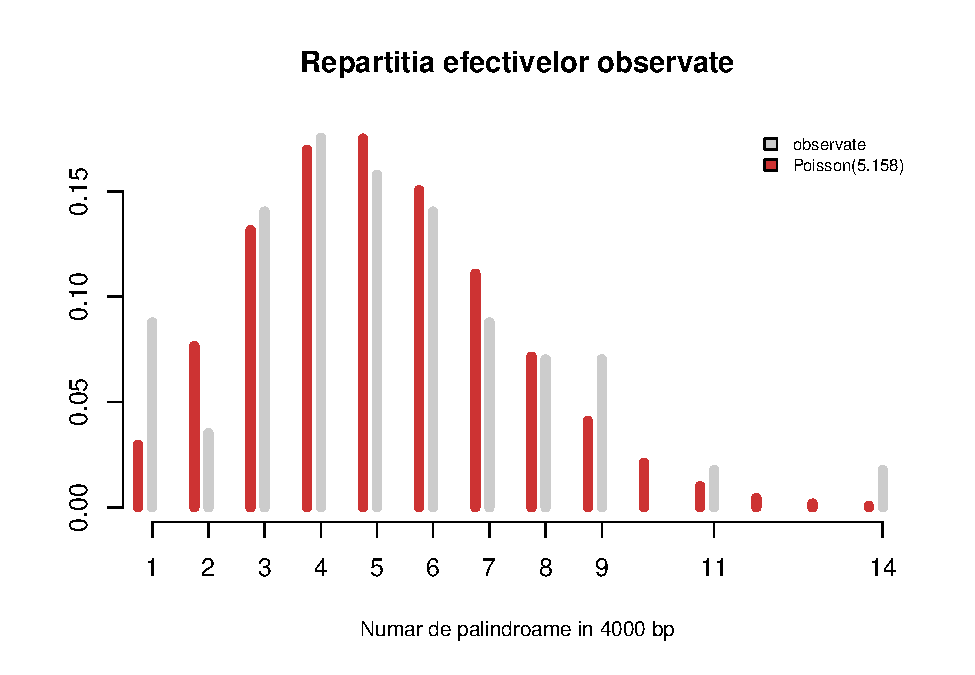
\includegraphics[width=0.8\linewidth]{Lab_5_files/figure-latex/unnamed-chunk-51-1} \end{center}

Pentru a calcula statistica de test \(\chi^2\) a lui Pearson avem

\[
X^2 = \sum_{j = 1}^{c}\frac{(O_{j} - E_{j})^2}{E_{j}} = \sum_{j = 1}^{c}\frac{\left(n_{j} - n \pi_j(\bar{\theta})\right)^2}{n \pi_j(\bar{\theta})}
\]

unde tabelul efectivelor observate și respectiv așteptate este
\rowcolors{2}{gray!6}{white}

\begin{longtable}{ccccccccc}
\hiderowcolors
\toprule
Interval & Efective observate & Efective asteptate\\
\midrule
\endfirsthead
\multicolumn{9}{@{}l}{\textit{(continued)}}\\
\toprule
Interval & Efective observate & Efective asteptate\\
\midrule
\endhead
\
\endfoot
\bottomrule
\endlastfoot
\showrowcolors
<=2 & 7 & 6.382176\\
3 & 8 & 7.500597\\
4 & 10 & 9.671822\\
5 & 9 & 9.977248\\
6 & 8 & 8.576932\\
\addlinespace
7 & 5 & 6.319845\\
8 & 4 & 4.074637\\
>=9 & 6 & 4.496744\\*
\end{longtable}

\rowcolors{2}{white}{white}

iar statistica de test devine \(X^2=\) 1.0182639.

P-valoarea testului este

\begin{Shaded}
\begin{Highlighting}[]
\NormalTok{observed =}\StringTok{ }\KeywordTok{c}\NormalTok{(}\KeywordTok{sum}\NormalTok{(counts }\OperatorTok\StringTok{ }\KeywordTok{c}\NormalTok{(}\DecValTok{1}\NormalTok{,}\DecValTok{2}\NormalTok{)),}
             \KeywordTok{sum}\NormalTok{(counts }\OperatorTok{==}\StringTok{ }\DecValTok{3}\NormalTok{), }
             \KeywordTok{sum}\NormalTok{(counts }\OperatorTok{==}\StringTok{ }\DecValTok{4}\NormalTok{),}
             \KeywordTok{sum}\NormalTok{(counts }\OperatorTok{==}\StringTok{ }\DecValTok{5}\NormalTok{),}
             \KeywordTok{sum}\NormalTok{(counts }\OperatorTok{==}\StringTok{ }\DecValTok{6}\NormalTok{),}
             \KeywordTok{sum}\NormalTok{(counts }\OperatorTok{==}\StringTok{ }\DecValTok{7}\NormalTok{),}
             \KeywordTok{sum}\NormalTok{(counts }\OperatorTok{==}\StringTok{ }\DecValTok{8}\NormalTok{),}
             \KeywordTok{sum}\NormalTok{(counts }\OperatorTok{>=}\StringTok{ }\DecValTok{9}\NormalTok{))}
\NormalTok{expected =}\StringTok{ }\NormalTok{n.int}\OperatorTok{*}\KeywordTok{c}\NormalTok{(}\KeywordTok{ppois}\NormalTok{(}\DecValTok{2}\NormalTok{, lambda), }
                      \KeywordTok{dpois}\NormalTok{(}\DecValTok{3}\OperatorTok{:}\DecValTok{8}\NormalTok{, lambda),}
                      \DecValTok{1} \OperatorTok{-}\StringTok{ }\KeywordTok{ppois}\NormalTok{(}\DecValTok{8}\NormalTok{, lambda))}

\NormalTok{X2 =}\StringTok{ }\KeywordTok{sum}\NormalTok{((observed }\OperatorTok{-}\StringTok{ }\NormalTok{expected)}\OperatorTok{^}\DecValTok{2}\OperatorTok{/}\NormalTok{expected)}

\CommentTok{# p-valoarea}
\DecValTok{1}\OperatorTok{-}\KeywordTok{pchisq}\NormalTok{(X2, }\KeywordTok{length}\NormalTok{(observed) }\OperatorTok{-}\StringTok{ }\DecValTok{2}\NormalTok{)}
\NormalTok{[}\DecValTok{1}\NormalTok{] }\FloatTok{0.9849105}
\end{Highlighting}
\end{Shaded}

și prin urmare nu putem respinge ipoteza nulă prin care repartiția
numărului de palindroame pe intervale de lungime 4000 de perechi de bază
este Poisson de medie \(\lambda=\) 5.158.

\section{\texorpdfstring{Tabele de contingență
\(r\times c\)}{Tabele de contingență r\textbackslash{}times c}}\label{tabele-de-contingenta-rtimes-c}

\subsection{Modelul multinomial}\label{modelul-multinomial}

În acest model, presupunem că vectorul aleator \((X,Y)\) ia valori în
\(\{x_1,\ldots, x_r\}\times\{y_1,\ldots, y_c\}\) și numărul total de
observații \(n\) (talia eșantionului) este fixat. Repartiția vectorului
\((X,Y)\) este

\[
  \mathbb{P}\circ(X,Y)^{-1} = \sum_{i = 1}^{r}\sum_{j = 1}^{c}p_{ij}\delta_{(x_i,y_j)},
\]

unde \(\mathbb{P}(X = x_i, Y = y_j) = p_{ij}\), iar repartițiile
marginale sunt

\begin{align*}
  \mathbb{P}\circ X^{-1} &= \sum_{i = 1}^{r}p_i\delta_{x_i},\quad \mathbb{P}(X = x_i) = p_{i},\, i\in\{1,2,\ldots,r\} \\
  \mathbb{P}\circ Y^{-1} &= \sum_{j = 1}^{c}q_j\delta_{y_j},\quad \mathbb{P}(Y = y_j) = q_{j},\, j\in\{1,2,\ldots,c\}.
\end{align*}

Tabelul de contingență se scrie

\[
\begin{array}{c|ccccc|c}
  X / Y  &  y_1      & \cdots &  y_j     & \cdots &  y_c     & \mathbb{P}\circ X^{-1}\\
  \hline
  x_1      &  p_{11} & \cdots & p_{1j} & \cdots & p_{1c} & p_{1}\\
  \vdots & \vdots  & \vdots & \vdots & \vdots & \vdots & \vdots  \\
  x_i      &  p_{i1} & \cdots & p_{ij} & \cdots & p_{ic} & p_{i}\\
  \vdots & \vdots  & \vdots & \vdots & \vdots & \vdots & \vdots  \\
  x_r      &  p_{r1} & \cdots & p_{rj} & \cdots & p_{rc} & p_{r}\\
  \hline
  \mathbb{P}\circ Y^{-1}&  q_{1} & \cdots & q_{j} & \cdots & q_{c} & 1\\
\end{array}
\]

Fie \((X_1,Y_1), \ldots, (X_n,Y_n)\) un eșantion de talie \(n\) din
populația \(\mathbb{P}\circ(X,Y)^{-1}\). Tabelul de contingență a
efectivelor observate este

\[
\begin{array}{c|ccccc|c}
  X / Y  &  y_1      & \cdots &  y_j     & \cdots &  y_c     & \sum\\
  \hline
  x_1      &  N_{11} & \cdots & N_{1j} & \cdots & N_{1c} & N_{1\cdot}\\
  \vdots & \vdots  & \vdots & \vdots & \vdots & \vdots & \vdots  \\
  x_i      &  N_{i1} & \cdots & N_{ij} & \cdots & N_{ic} & N_{i\cdot}\\
  \vdots & \vdots  & \vdots & \vdots & \vdots & \vdots & \vdots  \\
  x_r      &  N_{r1} & \cdots & N_{rj} & \cdots & N_{rc} & N_{r\cdot}\\
  \hline
  \sum   &  N_{\cdot 1} & \cdots & N_{\cdot j} & \cdots & N_{\cdot c} & n\\
\end{array}
\]

unde \(N_{ij} = \sum_{k = 1}^{n}\mathbf{1}_{(x_i, y_j)}(X_k,Y_k)\)
reprezintă numărul de observații din celula \((i,j)\). Notăm de asemenea
cu \(N_{i\cdot} = \sum_{j = 1}^{c}N_{ij}\),
\(N_{\cdot j} = \sum_{i = 1}^{r}N_{ij}\) și respectiv
\(n = \sum_{i = 1}^{r}\sum_{j = 1}^{c}N_{ij}\) (în acest model este
fixat). Pentru datele statistice (eșantionul observat)
\((x_1,y_1), \ldots, (x_n,y_n)\) vom folosi litere mici, i.e.
\(n{ij} = N_{ij}(\omega) = \sum_{k = 1}^{n}\mathbf{1}_{(x_i, y_j)}(X_k(\omega),Y_k(\omega))\).

În acest model, vrem să testăm independența variabilelor discrete
(calitative) \(X\) și \(Y\) (că nu există asociere între cele două
variabile):

\begin{align*}
  H_0: & \{\text{$X$ și $Y$ sunt independente}\} = \{\mathbb{P}(X = x_i, Y = y_j) = \mathbb{P}(X = x_i)\mathbb{P}(Y = y_j),\,\forall i,j\}\\
    & = \{p_{ij} = p_i q_j, \forall i,j\}\\
  H_1: & \{\text{$X$ și $Y$ nu sunt independente}\} = \{\exists i,j \; \mathbb{P}(X = x_i, Y = y_j) \neq \mathbb{P}(X = x_i)\mathbb{P}(Y = y_j)\}\\
    & = \{\exists i,j \; p_{ij} \neq p_i q_j\}
\end{align*}

Pentru aceasta vom folosi testul bazat pe raportul de verosimilitate

\[
  \Lambda(\mathbf{x})=\frac{\sup_{\theta\in\Theta_0}L(\theta|\mathbf{x})}{\sup_{\theta\in\Theta}L(\theta|\mathbf{x})},
\]

unde \(\Theta\) este spațiul parametrilor modelului, \(\Theta_0\) este
spațiul parametrilor corespunzător ipotezei nule iar
\(L(\theta|\mathbf{x})\) este funcția de verosimilitate.

Observăm că spațiul parametrilor corespunzător modelului este

\[
\Theta = \left\{(p_{11},\ldots, p_{1c},\ldots, p_{r1},\ldots,p_{rc}\,|\,p_{ij}\in(0,1),\,\sum_{i = 1}^{r}\sum_{j = 1}^{c}p_{ij} = 1\right\},
\]

cu \(\dim{\Theta} = rc-1\), cel corespunzător ipotezei nule este

\[
\Theta_0 = \left\{(p_{1}q_{1},\ldots, p_{1}q_{c},\ldots, p_{r}q_{1},\ldots,p_{r}q_{c}\,|\,p_{i}, q_{j}\in(0,1),\,\sum_{i = 1}^{r}p_{i} = 1,\, \sum_{j = 1}^{c}q_j = 1\right\}
\]

cu \(\dim{\Theta_0} = r+c-2\) iar funcția de verosimilitate
(probabilitatea să observăm tabelul
\(\mathbb{P}_{\theta}(\text{tabel})\)) este

\begin{align*}
  L(p_{ij},\,i = 1,\ldots, r,\, j = 1,\ldots,c\,;\,\mathbf{x}) &= \mathbb{P}(N_{ij} = n_{ij}, \,i = 1,\ldots, r,\, j = 1,\ldots,c) \\
    &= \frac{n!}{\prod_{i = 1}^{r}\prod_{j = 1}^{c} n_{ij}!}\prod_{i = 1}^{r}\prod_{j = 1}^{c} p_{ij}^{n_{ij}}\propto \prod_{i = 1}^{r}\prod_{j = 1}^{c} p_{ij}^{n_{ij}}.
\end{align*}

Pentru a determina estimatorul de verosimilitate maximă pe \(\Theta\)
trebuie să rezolvăm problema de optimizare:

\[
  \left\{\begin{array}{ll}
    \max_{\theta\in\Theta} \log L(\theta|\mathbf{x}) = \max \sum_{i = 1}^{r}\sum_{j = 1}^{c}n_{ij}\log{p_{ij}}\\
    \sum_{i = 1}^{r}\sum_{j = 1}^{c}p_{ij} = 1
  \end{array}\right.
\]

Aplicând metoda
\href{https://en.wikipedia.org/wiki/Lagrange_multiplier}{multiplicatorilor
lui Lagrange} avem funcția lui Lagrange

\[
\mathcal{L}(p_{ij},\,i = 1,\ldots, r,\, j = 1,\ldots,c\,;\lambda) = \sum_{i = 1}^{r}\sum_{j = 1}^{c}n_{ij}\log{p_{ij}} - \lambda\left(\sum_{i = 1}^{r}\sum_{j = 1}^{c}p_{ij} - 1\right)
\]

și rezolvând ecuația
\(\frac{\partial \mathcal{L}(p_{ij},\,i = 1,\ldots, r,\, j = 1,\ldots,c\,;\lambda)}{\partial p_{ij}} = 0\)
găsim

\[
\frac{\partial \mathcal{L}}{\partial p_{ij}} = 0 \iff \frac{n_{ij}}{p_{ij}} - \lambda = 0 \iff p_{ij} = \frac{n_{ij}}{\lambda},\forall i,j
\]

și din restricția \(\sum_{i = 1}^{r}\sum_{j = 1}^{c}p_{ij} = 1\) deducem
că \(\sum_{i = 1}^{r}\sum_{j = 1}^{c}\frac{n_{ij}}{\lambda} = 1\) de
unde \(\hat{\lambda} = n\), ceea ce conduce la soluția

\[
  \boxed{\hat{p}_{ij} = \frac{n_{ij}}{n}}.
\]

Sub ipoteza nulă, funcția de verosimilitate se scrie

\[
L(p_{i}, q_{j},\,i = 1,\ldots, r,\, j = 1,\ldots,c\,;\,\mathbf{x}) = \frac{n!}{\prod_{i = 1}^{r}\prod_{j = 1}^{c} n_{ij}!}\prod_{i = 1}^{r}\prod_{j = 1}^{c} (p_{i}q_{j})^{n_{ij}}\propto \prod_{i = 1}^{r}\prod_{j = 1}^{c} (p_{i}q_{j})^{n_{ij}}
\]

iar estimatorul de verosimilitate maximă sub \(\Theta_0\) impune
rezolvarea problemei de optimizare cu restricții

\[
  \left\{\begin{array}{ll}
    \max_{\theta\in\Theta_0} \log L(\theta|\mathbf{x}) = \max \sum_{i = 1}^{r}\sum_{j = 1}^{c}n_{ij}\log(p_{i}q_{j})\\
    \sum_{i = 1}^{r}p_{i} = 1,\\
    \sum_{j = 1}^{c}q_{j} = 1.
  \end{array}\right.
\]

Funcția lui Lagrange din metoda multiplicatorilor lui Lagrange se scrie

\[
\mathcal{L}(p_{i}, q_{j},\,i = 1,\ldots, r,\, j = 1,\ldots,c\,;\lambda_1, \lambda_2) = \sum_{i = 1}^{r}\sum_{j = 1}^{c}n_{ij}\log{p_{i}q_{j}} - \lambda_1\left(\sum_{i = 1}^{r}p_{i} - 1\right) - \lambda_2\left(\sum_{j = 1}^{c}q_{j} - 1\right)
\]

Observăm că ecuația \(\frac{\partial \mathcal{L}}{\partial p_{i}} = 0\)
este echivalentă cu

\[
\frac{\partial \mathcal{L}}{\partial p_{i}} = 0 \iff \sum_{i = 1}^{r}\frac{n_{ij}}{p_i} - \lambda_1 = 0 \iff p_{i} = \frac{n_{i\cdot}}{\lambda_1}
\]

și din restricția \(\sum_{i = 1}^{r}p_{i} = 1\) deducem că
\(\hat{\lambda}_1 = \sum_{i = 1}^{r}n_{i\cdot} = n\) iar
\(\boxed{\hat{p}_i = \frac{n_{i\cdot}}{n}}\).

În mod similar, din ecuația \(\frac{\partial \mathcal{L}}{q_{j}} = 0\)
și restricția \(\sum_{j = 1}^{c}q_{j} = 1\) găsim
\(\hat{\lambda}_2 = \sum_{j = 1}^{c}n_{\cdot j} = n\) iar
\(\boxed{\hat{q}_j = \frac{n_{\cdot j}}{n}}\).

Raportul de verosimilitate devine

\begin{align*}
  \Lambda(\mathbf{x})&=\frac{\sup_{\theta\in\Theta_0}L(\theta|\mathbf{x})}{\sup_{\theta\in\Theta}L(\theta|\mathbf{x})} = \frac{L(\hat{p}_i, \hat{q}_{j},,\,i = 1,\ldots, r,\, j = 1,\ldots,c)}{L(\hat{p}_{ij},\,i = 1,\ldots, r,\, j = 1,\ldots,c)}= \prod_{i = 1}^{r}\prod_{j = 1}^{c} \left(\frac{\hat{p}_{i}\hat{q}_{j}}{\hat{p}_{ij}}\right)^{n_{ij}} \\
  &= \prod_{i = 1}^{r}\prod_{j = 1}^{c} \left(\frac{n_{i\cdot}\times n_{\cdot j}}{n\times n_{ij}}\right)^{n_{ij}}
\end{align*}

și aplicând
\href{https://en.wikipedia.org/wiki/Likelihood-ratio_test}{Teorema lui
Wilks} avem

\[
  -2\log \Lambda(\mathbf{x}) = -2\sum_{i = 1}^{r}\sum_{j = 1}^{c} n_{ij}\log\left(\frac{n_{i\cdot}\times n_{\cdot j}}{n\times n_{ij}}\right) \underset{n\to\infty}{\overset{d}{\longrightarrow}}\chi^2(\underbrace{\dim{\Theta} - \dim{\Theta_0}}_{(rc-1)-(r+c-2)}) = \chi^2((r-1)(c-1))
\]

Prin urmare, regiunea critică a testului asimptotic de nivel \(\alpha\)
bazat pe raportul de verosimilitate este

\[
  C = \left\{\mathbf{x} \,|\, -2\log \Lambda(\mathbf{x}) > \chi^2_{1-\alpha}((r-1)(c-1))\right\}.
\]

Statistica testului \(\chi^2\) a lui Pearson este

\[
  X^2 = \sum_{i = 1}^{r}\sum_{j = 1}^{c}\frac{(O_{ij} - E_{ij})^2}{E_{ij}}
\]

unde \(O_{ij} = N_{ij}\) sunt efectivele observate iar \(E_{ij}\) sunt
efectivele pe care ne așteptăm să le observăm dacă ipoteza nulă ar fi
adevărată (sub \(H_0\), repartiția condiționată a lui \(N_{ij}\) la
\(\sum_{i = 1}^{r}\sum_{j = 1}^{c}N_{ij} = n\) este
\(\mathcal{B}(n,p_{ij})\)),

\[
  E_{ij} = \mathbb{E}_{H_0}[N_{ij}] = n \hat{p}_i \hat{q}_j = n \frac{N_{i\cdot}}{n}\frac{N_{\cdot j}}{n} = \frac{N_{i\cdot}N_{\cdot j}}{n}
\]

ceea ce implică

\[
  X^2 = \sum_{i = 1}^{r}\sum_{j = 1}^{c}\frac{\left(N_{ij} - \frac{N_{i\cdot}N_{\cdot j}}{n}\right)^2}{\frac{N_{i\cdot}N_{\cdot j}}{n}}.
\]

Această statistică este asimptotic repartizată

\[
  X^2 = \sum_{i = 1}^{r}\sum_{j = 1}^{c}\frac{\left(N_{ij} - \frac{N_{i\cdot}N_{\cdot j}}{n}\right)^2}{\frac{N_{i\cdot}N_{\cdot j}}{n}} \underset{n\to\infty}{\overset{d}{\longrightarrow}} \chi^2((r-1)(c-1))
\]

prin urmare testul \(\chi^2\) a lui Pearson de nivel \(\alpha\), pentru
ipotezele \(H_0\,vs\,H_1\) conduce la aceeași regiune critică ca și
testul bazat pe raportul de verosimilitate (cu toate acestea se poate
arăta că statistica lui Pearson \(X^2\) converge mai repede decât
statistica \(-2\log \Lambda(\mathbf{x})\), \citep{Agresti2012}).

\subsection{Modelul multinomial
independent}\label{modelul-multinomial-independent}

În acest model considerăm că \(Y\) este variabila răspuns iar \(X\) este
fixată (nu este o variabilă aleatoare), astfel încât fiecare categorie a
lui \(X\), \(\{X = x_i\}\) descrie populația \(i\).

Dată fiind o observație clasificată în categoria \(i\) a lui \(X\) (pe
rândul \(i\)) notăm cu \(p_{j|i}\) probabilitatea ca observația să se
afle în categoria \(j\) a lui \(Y\), cu alte cuvinte putem interpreta
probabilitățile \(\{p_{1|i}, p_{2|i}, \ldots, p_{c|i}\}\) ca repartiția
condiționată a lui \(Y\) la \(X = x_i\)
(\(p_{j|i} = \mathbb{P}(Y = y_j|X = x_i)\)).

Modelul multinomial independent (sau produs) presupune compararea mai
multor populații în care un număr predeterminat de observații este
eșantionat independent din fiecare populație, cu alte cuvinte compararea
repartițiilor condiționate ale lui \(Y\) pentru diverse categorii ale
lui \(X\).

Tabelul de contingență se scrie

\[
\begin{array}{c|ccccc|c}
  X / Y  &  y_1      & \cdots &  y_j     & \cdots &  y_c     & \sum\\
  \hline
  x_1      &  p_{1|1} & \cdots & p_{j|1} & \cdots & p_{c|1} & 1\\
  \vdots & \vdots  & \vdots & \vdots & \vdots & \vdots & \vdots  \\
  x_i      &  p_{1|i} & \cdots & p_{j|i} & \cdots & p_{c|i} & 1\\
  \vdots & \vdots  & \vdots & \vdots & \vdots & \vdots & \vdots  \\
  x_r      &  p_{1|r} & \cdots & p_{j|r} & \cdots & p_{c|r} & 1\\
  \hline
  \sum&  q_{1} & \cdots & q_{j} & \cdots & q_{c} & \\
\end{array}
\]

O observație din populația \(i\) poate fi modelată cu ajutorul
vectorului aleator
\(\mathbf{X}^{(i)} = (X_1^{(i)}, X_2^{(i)}, \ldots, X_c^{(i)})\) care
este repartizat \(\mathcal{M}(1;p_{1|i},p_{2|i},\ldots,,p_{c|i})\)
(fiecare observație este clasificată într-o singură categorie \(y_j\),
\(j\in\{1,2,\ldots,c\}\)). Fie eșantioanele independente
\(\mathbf{X}^{(1)}_1, \ldots, \mathbf{X}^{(1)}_{n_{1\cdot}}\),
\(\mathbf{X}^{(2)}_1, \ldots, \mathbf{X}^{(2)}_{n_{2\cdot}}\),
\(\cdots\),
\(\mathbf{X}^{(r)}_1, \ldots, \mathbf{X}^{(r)}_{n_{r\cdot}}\) de talie
\(n_{1\cdot}, n_{2\cdots}, \ldots, n_{r\cdot}\) din populațiile
\(X = x_1, X = x_2, \ldots, X = x_r\). Atunci tabelul de contingență a
efectivelor observate este

\[
\begin{array}{c|ccccc|c}
  X / Y  &  y_1      & \cdots &  y_j     & \cdots &  y_c     & \sum\\
  \hline
  x_1      &  N_{11} & \cdots & N_{1j} & \cdots & N_{1c} & n_{1\cdot}\\
  \vdots & \vdots  & \vdots & \vdots & \vdots & \vdots & \vdots  \\
  x_i      &  N_{i1} & \cdots & N_{ij} & \cdots & N_{ic} & n_{i\cdot}\\
  \vdots & \vdots  & \vdots & \vdots & \vdots & \vdots & \vdots  \\
  x_r      &  N_{r1} & \cdots & N_{rj} & \cdots & N_{rc} & n_{r\cdot}\\
  \hline
  \sum   &  N_{\cdot 1} & \cdots & N_{\cdot j} & \cdots & N_{\cdot c} & n\\
\end{array}
\]

unde
\(N_{ij} = = \sum_{k = 1}^{n_{i\cdot}}\mathbf{1}_{(0,\ldots, \underbrace{1}_{y_j},\ldots, 0)}(\mathbf{X}^{(i)}_k)\)
reprezintă numărul de observații din populația \(i\) care se află în
categoria \(Y = y_j\). Observăm că în acest model efectivele totale pe
linii, \(n_{i\cdot}\) sunt fixate.

În acest model vrem să testăm ipoteza de \emph{omogenitate} a
populațiilor și anume

\begin{align*}
  H_0: & \{\forall j = 1,2,\ldots, c \text{ avem } p_{j|i} = q_j, \forall i = 1,2,\ldots,r\}\\
    & = \left\{\begin{array}{llll}
      p_{1|1} = p_{2|1} = \cdots = p_{c|1} = q_1\\
      p_{1|2} = p_{2|2} = \cdots = p_{c|2} = q_2\\
      \cdots \cdots \cdots \cdots \cdots \\
      p_{1|r} = p_{2|r} = \cdots = p_{c|r} = q_r\\
    \end{array}\right.\\
  H_1: & \{\exists j, \exists i_1\neq i_2 \text{ astfel ca } p_{j|i_1}\neq p_{j|i_2}\} 
\end{align*}

unde \((q_1,\ldots, q_r)\) este repartiția comună a celor \(r\)
populații.

Ca și în modelul anterior vom folosi testul bazat pe raportul de
verosimilitate

\[
  \Lambda(\mathbf{x})=\frac{\sup_{\theta\in\Theta_0}L(\theta|\mathbf{x})}{\sup_{\theta\in\Theta}L(\theta|\mathbf{x})},
\]

unde \(\Theta\) este spațiul parametrilor modelului, \(\Theta_0\) este
spațiul parametrilor corespunzător ipotezei nule iar
\(L(\theta|\mathbf{x})\) este funcția de verosimilitate.

Observăm că spațiul parametrilor corespunzător modelului este

\[
\Theta = \left\{(p_{1|1},\ldots, p_{c|1},\ldots, p_{1|r},\ldots,p_{c|r}\,|\,p_{j|i}\in(0,1),\,\sum_{j = 1}^{c}p_{j|i} = 1, \forall i = 1,\ldots,r\right\},
\]

cu \(\dim{\Theta} = rc-r\), cel corespunzător ipotezei nule este

\[
\Theta_0 = \left\{(q_{1},\ldots, q_{c},\ldots, q_{1},\ldots,q_{c}\,|\,q_{j}\in(0,1),\,\sum_{j = 1}^{c}q_j = 1\right\}
\]

cu \(\dim{\Theta_0} = c-1\) iar funcția de verosimilitate
(probabilitatea să observăm tabelul
\(\mathbb{P}_{\theta}(\text{tabel})\)) este

\begin{align*}
  L(p_{j|i},\,i = 1,\ldots, r,\, j = 1,\ldots,c\,;\,\mathbf{x}) &= \mathbb{P}(\forall i = 1,\ldots, r,\, N_{ij} = n_{ij},\forall j = 1,\ldots,c) \\
    &= \prod_{i = 1}^{r}\mathbb{P}(N_{ij} = n_{ij},\, j = 1,\ldots,c) = \prod_{i = 1}^{r}\left[\frac{n_{i\cdot}!}{\prod_{j = 1}^{c}n_{ij}!}\prod_{j = 1}^{c} p_{j|i}^{n_{ij}}\right]\\
    & = \frac{\prod_{i = 1}^{r}n_{i\cdot}!}{\prod_{i = 1}^{r}\prod_{j = 1}^{c} n_{ij}!}\prod_{i = 1}^{r}\prod_{j = 1}^{c} p_{j|i}^{n_{ij}}\propto
    \prod_{i = 1}^{r}\prod_{j = 1}^{c} p_{j|i}^{n_{ij}}.
\end{align*}

Pentru a determina \(\sup_{\theta\in\Theta}L(\theta|\mathbf{x})\)
trebuie să determinăm estimatorul de verosimilitate maximă pe
\(\Theta\), deci ne propunem să rezolvăm problema de optimizare:

\[
  \left\{\begin{array}{ll}
    \max_{\theta\in\Theta} \log L(\theta|\mathbf{x}) = \max \sum_{i = 1}^{r}\sum_{j = 1}^{c}n_{ij}\log{p_{j|i}}\\
    \sum_{j = 1}^{c}p_{ij} = 1, \, i = 1,\ldots,r
  \end{array}\right.
\]

Ca și în problemele de optimizare din modelul multinomial vom folosi
metoda
\href{https://en.wikipedia.org/wiki/Lagrange_multiplier}{multiplicatorilor
lui Lagrange}. Avem funcția lui Lagrange

\[
\mathcal{L}(p_{1|i},\ldots, p_{c|i},\,i = 1,\ldots, r\,;\lambda_1,\ldots,\lambda_r) = \sum_{i = 1}^{r}\sum_{j = 1}^{c}n_{ij}\log{p_{j|i}} - \sum_{i = 1}^{r}\lambda_i\left(\sum_{j = 1}^{c}p_{j|i} - 1\right)
\]

și rezolvând ecuațiile
\(\frac{\partial \mathcal{L}}{\partial p_{j|i}} = 0\), pentru
\(i = 1,2,\ldots,r\), găsim

\[
\frac{\partial \mathcal{L}}{\partial p_{j|i}} = 0 \iff \frac{n_{ij}}{p_{j|i}} - \lambda_i = 0 \iff p_{j|i} = \frac{n_{ij}}{\lambda_i},\forall j = 1,2,\ldots,c
\]

Folosind cele \(r\) restricții \(\sum_{j = 1}^{c}p_{j|i} = 1\) deducem
că \(\sum_{j = 1}^{c}\frac{n_{ij}}{\lambda_i} = 1\) de unde
\(\hat{\lambda}_i = n_{i\cdot}\), ceea ce conduce la soluția

\[
  \boxed{\hat{p}_{j|i} = \frac{n_{ij}}{n_{i\cdot}}}.
\]

În mod similar, pentru a determina
\(\sup_{\theta\in\Theta_0}L(\theta|\mathbf{x})\) trebuie să găsim
estimatorul de verosimilitate maximă pe \(\Theta_0\). Sub ipoteza nulă,
funcția de verosimilitate se scrie

\[
L(q_{j},\, j = 1,\ldots,c\,;\,\mathbf{x}) = \frac{\prod_{i = 1}^{r}n_{i\cdot}!}{\prod_{i = 1}^{r}\prod_{j = 1}^{c} n_{ij}!}\prod_{i = 1}^{r}\prod_{j = 1}^{c} q_{j}^{n_{ij}} = \frac{\prod_{i = 1}^{r}n_{i\cdot}!}{\prod_{i = 1}^{r}\prod_{j = 1}^{c} n_{ij}!}\prod_{j = 1}^{c} q_{j}^{n_{\cdot j}}\propto \prod_{j = 1}^{c} q_{j}^{n_{\cdot j}}
\]

iar estimatorul de verosimilitate maximă sub \(\Theta_0\) impune
rezolvarea problemei de optimizare cu restricții

\[
  \left\{\begin{array}{ll}
    \max_{\theta\in\Theta_0} \log L(\theta|\mathbf{x}) = \max \sum_{j = 1}^{c}n_{\cdot j}\log{q_{j}}\\
    \sum_{j = 1}^{c}q_{j} = 1
  \end{array}\right.
\]

Funcția lui Lagrange din metoda multiplicatorilor lui Lagrange se scrie

\[
\mathcal{L}(q_{j},\, j = 1,\ldots,c\,;\lambda) = \sum_{j = 1}^{c}n_{\cdot j}\log{q_{j}} - \lambda\left(\sum_{j = 1}^{c}q_{j} - 1\right)
\]

Observăm că ecuația \(\frac{\partial \mathcal{L}}{\partial q_{j}} = 0\)
este echivalentă cu

\[
\frac{\partial \mathcal{L}}{\partial q_{j}} = 0 \iff \frac{n_{\cdot j}}{q_j} - \lambda = 0 \iff q_{j} = \frac{n_{\cdot j}}{\lambda}, \, j =1,2,\ldots,c
\]

și din restricția \(\sum_{j = 1}^{c}q_{j} = 1\) deducem că
\(\hat{\lambda} = \sum_{j = 1}^{c}n_{\cdot j} = n\) iar
\(\boxed{\hat{q}_j = \frac{n_{\cdot j}}{n}}\).

Raportul de verosimilitate devine

\begin{align*}
  \Lambda(\mathbf{x})&=\frac{\sup_{\theta\in\Theta_0}L(\theta|\mathbf{x})}{\sup_{\theta\in\Theta}L(\theta|\mathbf{x})} = \frac{L(\hat{p}_{1|i},\ldots, \hat{p}_{c|i},\,i = 1,\ldots, r)}{L(\hat{q}_{j},\, j = 1,\ldots,c)}= \prod_{i = 1}^{r}\prod_{j = 1}^{c} \left(\frac{\hat{q}_{j}}{\hat{p}_{j|i}}\right)^{n_{ij}} \\
  &= \prod_{i = 1}^{r}\prod_{j = 1}^{c} \left(\frac{n_{i\cdot}\times n_{\cdot j}}{n\times n_{ij}}\right)^{n_{ij}}
\end{align*}

și aplicând
\href{https://en.wikipedia.org/wiki/Likelihood-ratio_test}{Teorema lui
Wilks} avem

\[
  -2\log \Lambda(\mathbf{x}) = -2\sum_{i = 1}^{r}\sum_{j = 1}^{c} n_{ij}\log\left(\frac{n_{i\cdot}\times n_{\cdot j}}{n\times n_{ij}}\right) \underset{n\to\infty}{\overset{d}{\longrightarrow}}\chi^2(\underbrace{\dim{\Theta} - \dim{\Theta_0}}_{(rc-r)-(c-1)}) = \chi^2((r-1)(c-1))
\] Prin urmare, regiunea critică a testului asimptotic de nivel
\(\alpha\) bazat pe raportul de verosimilitate este

\[
  C = \left\{\mathbf{x} \,|\, -2\log \Lambda(\mathbf{x}) > \chi^2_{1-\alpha}((r-1)(c-1))\right\}.
\]

Statistica testului \(\chi^2\) a lui Pearson este

\[
  X^2 = \sum_{i = 1}^{r}\sum_{j = 1}^{c}\frac{(O_{ij} - E_{ij})^2}{E_{ij}}
\]

unde \(O_{ij} = N_{ij}\) sunt efectivele observate iar \(E_{ij}\) sunt
efectivele pe care ne așteptăm să le observăm dacă ipoteza nulă ar fi
adevărată (sub \(H_0\), repartiția condiționată a lui \(N_{ij}\) la
\(\sum_{j = 1}^{c}N_{ij} = n_{i\cdot}\) este
\(\mathcal{B}(n_{i\cdot},q_{j})\)),

\[
  E_{ij} = \mathbb{E}_{H_0}[N_{ij}] = n_{i\cdot} \hat{q}_j = n_{i\cdot}\frac{N_{\cdot j}}{n} = \frac{n_{i\cdot}N_{\cdot j}}{n}
\]

ceea ce implică

\[
  X^2 = \sum_{i = 1}^{r}\sum_{j = 1}^{c}\frac{\left(N_{ij} - \frac{n_{i\cdot}N_{\cdot j}}{n}\right)^2}{\frac{n_{i\cdot}N_{\cdot j}}{n}}.
\]

Sub \(H_0\) avem că
\(X^2\underset{n\to\infty}{\overset{d}{\longrightarrow}} \chi^2((r-1)(c-1))\)
ceea ce arată că testul \(\chi^2\) a lui Pearson de nivel \(\alpha\),
pentru ipotezele \(H_0\,vs\,H_1\) are aceeași regiune critică ca și
testul bazat pe raportul de verosimilitate.

\subsection{Modelul Poisson}\label{modelul-poisson}

În acest model considerăm că numărul de observații din fiecare celulă
\((i,j)\) este modelat cu ajutorul unor variabile aleatoare independente
\(N_{ij}\) repartizate Poisson \(Pois(\mu_{ij})\) de medie \(\mu_{ij}\).

Tabelul de contingență a efectivelor observate este

\[
\begin{array}{c|ccccc|c}
  X / Y  &  y_1      & \cdots &  y_j     & \cdots &  y_c     & \sum\\
  \hline
  x_1      &  N_{11} & \cdots & N_{1j} & \cdots & N_{1c} & N_{1\cdot}\\
  \vdots & \vdots  & \vdots & \vdots & \vdots & \vdots & \vdots  \\
  x_i      &  N_{i1} & \cdots & N_{ij} & \cdots & N_{ic} & N_{i\cdot}\\
  \vdots & \vdots  & \vdots & \vdots & \vdots & \vdots & \vdots  \\
  x_r      &  N_{r1} & \cdots & N_{rj} & \cdots & N_{rc} & N_{r\cdot}\\
  \hline
  \sum   &  N_{\cdot 1} & \cdots & N_{\cdot j} & \cdots & N_{\cdot c} & N\\
\end{array}
\]

și cum \(N_{ij}\) sunt independente deducem că
\(\sum_{i = 1}^{r}\sum_{j = 1}^{c}N_{ij}\sim Pois(\sum_{i = 1}^{r}\sum_{j = 1}^{c}\mu_{ij})\)
iar

\scriptsize

\begin{align*}
  \mathbb{P}(N_{ij} = n_{ij},\,i = 1,\ldots, r,\, j = 1,\ldots,c\,|\,\sum_{i = 1}^{r}\sum_{j = 1}^{c}N_{ij} = n) &= \frac{\mathbb{P}(N_{ij} = n_{ij},\,i = 1,\ldots, r,\, j = 1,\ldots,c,\,\sum_{i = 1}^{r}\sum_{j = 1}^{c}n_{ij} = n)}{\mathbb{P}(\sum_{i = 1}^{r}\sum_{j = 1}^{c}N_{ij} = n)}\\
  &= \frac{\prod_{i = 1}^{r}\prod_{j = 1}^{c}\mathbb{P}(N_{ij} = n_{ij})}{\mathbb{P}(\sum_{i = 1}^{r}\sum_{j = 1}^{c}N_{ij} = n)} = \frac{\prod_{i = 1}^{r}\prod_{j = 1}^{c}e^{-\mu_{ij}}\frac{\mu_{ij}^{n_{ij}}}{n_{ij}!}}{e^{-\sum_{i = 1}^{r}\sum_{j = 1}^{c}\mu_{ij}}\frac{\left(\sum_{i = 1}^{r}\sum_{j = 1}^{c}\mu_{ij}\right)^{n}}{n!}}\\
  &= \frac{n!}{\prod_{i = 1}^{r}\prod_{j = 1}^{c}n_{ij}!}\prod_{i = 1}^{r}\prod_{j = 1}^{c}\left(\frac{\mu_{ij}}{\sum_{i = 1}^{r}\sum_{j = 1}^{c}\mu_{ij}}\right)^{n_{ij}}.
\end{align*}

\normalsize

Dacă notăm cu \(\mu = \sum_{i = 1}^{r}\sum_{j = 1}^{c}\mu_{ij}\),
\(\mu_{i\cdot}=\sum_{j = 1}^{c}\mu_{ij}\) și respectiv
\(\mu_{\cdot j} = \sum_{i = 1}^{r}\mu_{ij}\) atunci putem considera
\(p_{ij} = \frac{\mu_{ij}}{\mu}\), \(p_{i} = \frac{\mu_{i\cdot}}{\mu}\)
și respectiv \(q_{j} = \frac{\mu_{\cdot j}}{\mu}\). În acest caz
condiția \(p_{ij} = p_{i}q_{j}\) se traduce în
\(\mu_{ij} = \frac{\mu_{i\cdot}\times \mu_{\cdot j}}{\mu}\), prin urmare
în acest model vrem să testăm ipotezele

\begin{align*}
  H_0: & \{\mu_{ij} = \frac{\mu_{i\cdot}\times \mu_{\cdot j}}{\mu}, \forall i = 1,2,\ldots,r,\,\forall j = 1,2,\ldots, c\}\\
  H_1: & \{\exists i, j \text{ astfel ca } \mu_{ij} \neq \frac{\mu_{i\cdot}\times \mu_{\cdot j}}{\mu}\} 
\end{align*}

și pentru aceasta, ca și în cazul modelelor anterioare, vom folosi
testul bazat pe raportul de verosimilitate

\[
  \Lambda(\mathbf{x})=\frac{\sup_{\theta\in\Theta_0}L(\theta|\mathbf{x})}{\sup_{\theta\in\Theta}L(\theta|\mathbf{x})},
\]

unde \(\Theta\) este spațiul parametrilor modelului, \(\Theta_0\) este
spațiul parametrilor corespunzător ipotezei nule iar
\(L(\theta|\mathbf{x})\) este funcția de verosimilitate.

Din definiția modelului observăm că spațiul parametrilor este

\[
\Theta = \left\{\mu_{ij},\,i = 1,\ldots,r,\,j = 1,\ldots,c\right\},
\]

cu \(\dim{\Theta} = rc\), cel corespunzător ipotezei nule este

\[
\Theta_0 = \left\{\frac{\mu_{i\cdot}\times \mu_{\cdot j}}{\mu},\, i = 1,2,\ldots,r,\,j = 1,2,\ldots, c\,|\,\sum_{i = 1}^{r}\mu_{i\cdot} = \mu,\,\sum_{j = 1}^{c}\mu_{\cdot j} = \mu\right\}
\]

cu \(\dim{\Theta_0} = r+c+1-2\) iar funcția de verosimilitate
(probabilitatea să observăm tabelul
\(\mathbb{P}_{\theta}(\text{tabel})\)) este

\begin{align*}
  L(\mu_{ij},\,i = 1,\ldots, r,\, j = 1,\ldots,c\,;\,\mathbf{x}) &= \mathbb{P}(N_{ij} = n_{ij},\forall j = 1,\ldots,c,\, \forall i = 1,\ldots, r) \\
    &= \prod_{i = 1}^{r}\prod_{j = 1}^{c}\mathbb{P}(N_{ij} = n_{ij}) = \prod_{i = 1}^{r}\prod_{j = 1}^{c}e^{-\mu_{ij}}\frac{\mu_{ij}^{n_{ij}}}{n_{ij}!}\\
    &\propto \prod_{i = 1}^{r}\prod_{j = 1}^{c}e^{-\mu_{ij}}\mu_{ij}^{n_{ij}}.
\end{align*}

Observăm că estimatorul de verosimilitate maximă pe \(\Theta\) presupune
maximizarea logaritmului funcției de verosimilitate

\[
\log L(\theta|\mathbf{x}) = \sum_{i = 1}^{r}\sum_{j = 1}^{c}(n_{ij}\log{\mu_{ij}} - \mu_{ij})
\]

iar ecuația de verosimilitate conduce la

\[
\frac{\partial \log{L}}{\partial \mu_{ij}} = 0 \iff \frac{n_{ij}}{\mu_{ij}} - 1 = 0 \iff \boxed{\hat{\mu}_{ij} = n_{ij}}.
\]

Pentru a determina \(\sup_{\theta\in\Theta_0}L(\theta|\mathbf{x})\)
trebuie să găsim estimatorul de verosimilitate maximă pe \(\Theta_0\).
Sub ipoteza nulă, funcția de verosimilitate se scrie

\[
L\left(\frac{\mu_{i\cdot}\times \mu_{\cdot j}}{\mu},\, i = 1,\ldots,r,\,j = 1,\ldots, c\,;\,\mathbf{x}\right) = \prod_{i = 1}^{r}\prod_{j = 1}^{c}e^{-\frac{\mu_{i\cdot}\times \mu_{\cdot j}}{\mu}}\frac{\left(\frac{\mu_{i\cdot}\times \mu_{\cdot j}}{\mu}\right)^{n_{ij}}}{n_{ij}!}\propto \prod_{i = 1}^{r}\prod_{j = 1}^{c}e^{-\frac{\mu_{i\cdot}\times \mu_{\cdot j}}{\mu}}\left(\frac{\mu_{i\cdot}\times \mu_{\cdot j}}{\mu}\right)^{n_{ij}}
\]

iar estimatorul de verosimilitate maximă sub \(\Theta_0\) impune
rezolvarea problemei de optimizare cu restricții

\[
  \left\{\begin{array}{lll}
    \max_{\theta\in\Theta_0} \log L(\theta|\mathbf{x}) = \max \sum_{i = 1}^{r}\sum_{j = 1}^{c}\left(n_{ij}\log{\frac{\mu_{i\cdot}\times \mu_{\cdot j}}{\mu}} - \frac{\mu_{i\cdot}\times \mu_{\cdot j}}{\mu}\right)\\
    \sum_{i = 1}^{r}\mu_{i\cdot} = \mu,\\
    \sum_{j = 1}^{c}\mu_{\cdot j} = \mu
  \end{array}\right.
\]

Ținând cont de restricții, observăm că ecuația
\(\frac{\partial \log{L}}{\partial \mu_{i\cdot}} = 0\) implică

\[
\frac{\partial \log{L}}{\partial \mu_{i\cdot}} = 0 \iff \sum_{j = 1}^{c}\left(\frac{n_{ij}}{\mu_{i\cdot}} - \frac{\mu_{\cdot j}}{\mu}\right) = 0 \iff \frac{n_{i\cdot}}{\mu_{i\cdot}} - 1 = 0 \iff \boxed{\hat{\mu}_{i\cdot} = n_{i\cdot}},
\]

iar ecuația \(\frac{\partial \log{L}}{\partial \mu_{\cdot j}} = 0\)
conduce la

\[
\frac{\partial \log{L}}{\partial \mu_{\cdot j}} = 0 \iff \sum_{i = 1}^{r}\left(\frac{n_{ij}}{\mu_{\cdot j}} - \frac{\mu_{i\cdot}}{\mu}\right) = 0 \iff \frac{n_{\cdot j}}{\mu_{\cdot j}} - 1 = 0 \iff \boxed{\hat{\mu}_{\cdot j} = n_{\cdot j}}.
\]

De asemenea, observăm că rezolvarea ecuației
\(\frac{\partial \log{L}}{\partial \mu} = 0\) implică

\[
\frac{\partial \log{L}}{\partial \mu} = 0 \iff -\sum_{i = 1}^{r}\sum_{j = 1}^{c}\frac{n_{ij}}{\mu} + \sum_{i = 1}^{r}\sum_{j = 1}^{c}\frac{\mu_{i\cdot}\times \mu_{\cdot j}}{\mu^2} = 0 \iff -\frac{n}{\mu} + 1 = 0 \iff \boxed{\hat{\mu} = n}
\]

iar
\(\boxed{\hat{\mu}_{ij} = \frac{\hat{\mu}_{i\cdot}\times \hat{\mu}_{\cdot j}}{\hat{\mu}} = \frac{n_{i\cdot}\times n_{\cdot j}}{n}}\).

Astfel, raportul de verosimilitate devine

\begin{align*}
  \Lambda(\mathbf{x})&=\frac{\sup_{\theta\in\Theta_0}L(\theta|\mathbf{x})}{\sup_{\theta\in\Theta}L(\theta|\mathbf{x})} = \frac{L(\hat{\mu}_{ij},\,i = 1,\ldots,r,\,j = 1,\ldots,c)}{L\left(\frac{\hat{\mu}_{i\cdot}\times \hat{\mu}_{\cdot j}}{\hat{\mu}},\, i = 1,2,\ldots,r,\,j = 1,2,\ldots, c\,;\,\mathbf{x}\right)}\\
  &= \frac{\prod_{i = 1}^{r}\prod_{j = 1}^{c}e^{-\frac{n_{i\cdot}\times n_{\cdot j}}{n}}\frac{1}{n_{ij}!}\left(\frac{n_{i\cdot}\times n_{\cdot j}}{n}\right)^{n_{ij}}}{\prod_{i = 1}^{r}\prod_{j = 1}^{c}e^{-n_{ij}}\frac{\mu_{ij}^{n_{ij}}}{n_{ij}!}}\\
  &= \prod_{i = 1}^{r}\prod_{j = 1}^{c}\left(\frac{\frac{n_{i\cdot}\times n_{\cdot j}}{n}}{n_{ij}}\right)^{n_{ij}} = \prod_{i = 1}^{r}\prod_{j = 1}^{c}\left(\frac{n_{i\cdot}\times n_{\cdot j}}{n\times n_{ij}}\right)^{n_{ij}}
\end{align*}

unde am folosit faptul că
\(\sum_{i = 1}^{r}\sum_{j = 1}^{c}\left(n_{ij} - \frac{n_{i\cdot}\times n_{\cdot j}}{n}\right) = 0\).
Aplicând
\href{https://en.wikipedia.org/wiki/Likelihood-ratio_test}{Teorema lui
Wilks} găsim că

\[
  -2\log \Lambda(\mathbf{x}) = -2\sum_{i = 1}^{r}\sum_{j = 1}^{c} n_{ij}\log\left(\frac{n_{i\cdot}\times n_{\cdot j}}{n\times n_{ij}}\right) \underset{n\to\infty}{\overset{d}{\longrightarrow}}\chi^2(\underbrace{\dim{\Theta} - \dim{\Theta_0}}_{(rc)-(r+c+1-2)}) = \chi^2((r-1)(c-1))
\] Prin urmare, regiunea critică a testului asimptotic de nivel
\(\alpha\) bazat pe raportul de verosimilitate este

\[
  C = \left\{\mathbf{x} \,|\, -2\log \Lambda(\mathbf{x}) > \chi^2_{1-\alpha}((r-1)(c-1))\right\}.
\]

\subsection{Aplicație}\label{aplicatie}

\begin{rmdexercise}
Următorul tabel prezintă repartiția grupelor de sânge (A, B, AB și O) în
trei eșantioane de cetățeni afro-americani care trăiesc în trei state
diferite (Florida, Iowa și Missouri). Vrem să testăm la un nivel de
semnificație \(\alpha = 0.05\) dacă repartiția grupelor de sânge pentru
cetățenii afro-americani diferă de-a lungul celor trei state.
\end{rmdexercise}

Suntem în cazul modelului multinomial independent și tabelul de
contingență este:

\rowcolors{2}{gray!6}{white}

\begin{longtable}{lcccccccccccccccccccc}
\hiderowcolors
\toprule
  & A & B & AB & O & Total\\
\midrule
\endfirsthead
\multicolumn{21}{@{}l}{\textit{(continued)}}\\
\toprule
  & A & B & AB & O & Total\\
\midrule
\endhead
\
\endfoot
\bottomrule
\endlastfoot
\showrowcolors
Florida & 122 & 117 & 19 & 244 & 502\\
Iowa & 1781 & 1351 & 288 & 3301 & 6721\\
Missouri & 353 & 269 & 60 & 713 & 1395\\
Total & 2256 & 1737 & 367 & 4258 & 8618\\*
\end{longtable}

\rowcolors{2}{white}{white}

\subsubsection{\texorpdfstring{Testul \(\chi^2\) al lui
Pearson}{Testul \textbackslash{}chi\^{}2 al lui Pearson}}\label{testul-chi2-al-lui-pearson}

Tabelul pe care ne așteptăm să-l observăm atunci când ipoteza nulă este
adevărată este:

\begin{Shaded}
\begin{Highlighting}[]
\NormalTok{  matAA_observed =}\StringTok{ }\KeywordTok{rbind}\NormalTok{(}\KeywordTok{c}\NormalTok{(}\DecValTok{122}\NormalTok{, }\DecValTok{117}\NormalTok{, }\DecValTok{19}\NormalTok{, }\DecValTok{244}\NormalTok{),}
           \KeywordTok{c}\NormalTok{(}\DecValTok{1781}\NormalTok{, }\DecValTok{1351}\NormalTok{, }\DecValTok{288}\NormalTok{, }\DecValTok{3301}\NormalTok{),}
           \KeywordTok{c}\NormalTok{(}\DecValTok{353}\NormalTok{, }\DecValTok{269}\NormalTok{, }\DecValTok{60}\NormalTok{, }\DecValTok{713}\NormalTok{))}

\NormalTok{  rs =}\StringTok{ }\KeywordTok{rowSums}\NormalTok{(matAA_observed) }
\NormalTok{  cs =}\StringTok{ }\KeywordTok{colSums}\NormalTok{(matAA_observed) }
  
\NormalTok{  n =}\StringTok{ }\KeywordTok{sum}\NormalTok{(matAA_observed)}
  
\NormalTok{  matAA_expected <-}\StringTok{ }\KeywordTok{outer}\NormalTok{(rs,cs,}\StringTok{"*"}\NormalTok{)}\OperatorTok{/}\NormalTok{n}
\end{Highlighting}
\end{Shaded}

\rowcolors{2}{gray!6}{white}

\begin{longtable}{lcccccccccccccccccccc}
\hiderowcolors
\toprule
  & A & B & AB & O & Total\\
\midrule
\endfirsthead
\multicolumn{21}{@{}l}{\textit{(continued)}}\\
\toprule
  & A & B & AB & O & Total\\
\midrule
\endhead
\
\endfoot
\bottomrule
\endlastfoot
\showrowcolors
Florida & 131.4124 & 101.1806 & 21.37781 & 248.0292 & 502\\
Iowa & 1759.4078 & 1354.6504 & 286.21571 & 3320.7262 & 6721\\
Missouri & 365.1799 & 281.1691 & 59.40647 & 689.2446 & 1395\\
Total & 2256.0000 & 1737.0000 & 367.00000 & 4258.0000 & 8618\\*
\end{longtable}

\rowcolors{2}{white}{white}

Aplicând funcția \texttt{chisq.test} obținem:

\begin{Shaded}
\begin{Highlighting}[]
\KeywordTok{chisq.test}\NormalTok{(matAA_observed)}

\NormalTok{    Pearson}\StringTok{'s Chi-squared test}

\StringTok{data:  matAA_observed}
\StringTok{X-squared = 5.6382, df = 6, p-value = 0.4649}
\end{Highlighting}
\end{Shaded}

\subsubsection{Testul bazat pe raportul de
verosimilități}\label{testul-bazat-pe-raportul-de-verosimilitati}

Aplicând funcția \texttt{LRT1} construită anterior

\begin{Shaded}
\begin{Highlighting}[]
\NormalTok{LRT1 =}\StringTok{ }\ControlFlowTok{function}\NormalTok{(dat)\{}
  \CommentTok{# dat este sub forma de matrice }
\NormalTok{  rs =}\StringTok{ }\KeywordTok{rowSums}\NormalTok{(dat) }\CommentTok{# apply(dat, 1, sum)}
\NormalTok{  cs =}\StringTok{ }\KeywordTok{colSums}\NormalTok{(dat) }\CommentTok{# apply(dat, 2, sum)}
  
\NormalTok{  n =}\StringTok{ }\KeywordTok{sum}\NormalTok{(dat)}
  
\NormalTok{  expected <-}\StringTok{ }\KeywordTok{outer}\NormalTok{(rs,cs,}\StringTok{"*"}\NormalTok{)}\OperatorTok{/}\NormalTok{n}
  
\NormalTok{  lrt <-}\StringTok{ }\OperatorTok{-}\DecValTok{2}\OperatorTok{*}\KeywordTok{sum}\NormalTok{(dat }\OperatorTok{*}\StringTok{ }\KeywordTok{log}\NormalTok{(expected}\OperatorTok{/}\NormalTok{dat)) }
  
\NormalTok{  dm =}\StringTok{ }\KeywordTok{dim}\NormalTok{(dat) }\CommentTok{# dimensiunea tabloului pentru a calcula gradele de libertate}
\NormalTok{  pval =}\StringTok{ }\DecValTok{1}\OperatorTok{-}\KeywordTok{pchisq}\NormalTok{(lrt,(dm[}\DecValTok{1}\NormalTok{]}\OperatorTok{-}\DecValTok{1}\NormalTok{)}\OperatorTok{*}\NormalTok{(dm[}\DecValTok{2}\NormalTok{]}\OperatorTok{-}\DecValTok{1}\NormalTok{))}
  
  \KeywordTok{cat}\NormalTok{(}\StringTok{"Statistica LRT este "}\NormalTok{, lrt, }\StringTok{"}\CharTok{\textbackslash{}n}\StringTok{"}\NormalTok{)}
  \KeywordTok{cat}\NormalTok{(}\StringTok{"P-valoarea testului bazat pe raportul de verosimilitate este "}\NormalTok{, pval)}
  
  \KeywordTok{return}\NormalTok{(}\KeywordTok{list}\NormalTok{(}\DataTypeTok{statistic =}\NormalTok{ lrt, }\DataTypeTok{pvalue =}\NormalTok{ pval))}
\NormalTok{\}}
\end{Highlighting}
\end{Shaded}

obținem p-valoarea testului bazat pe raportul de verosimilitate:

\begin{Shaded}
\begin{Highlighting}[]
\KeywordTok{LRT1}\NormalTok{(matAA_observed)}
\NormalTok{Statistica LRT este  }\FloatTok{5.548169} 
\NormalTok{P}\OperatorTok{-}\NormalTok{valoarea testului bazat pe raportul de verosimilitate este  }\FloatTok{0.475654}
\OperatorTok{$}\NormalTok{statistic}
\NormalTok{[}\DecValTok{1}\NormalTok{] }\FloatTok{5.548169}

\OperatorTok{$}\NormalTok{pvalue}
\NormalTok{[}\DecValTok{1}\NormalTok{] }\FloatTok{0.475654}
\end{Highlighting}
\end{Shaded}

\subsubsection{Testul aproximat al lui
Fisher}\label{testul-aproximat-al-lui-fisher}

Testul exact al lui Fisher poate fi aplicat și în cazul tabelelor de tip
\(r\times c\) (pentru o generalizare a testului prezentat la curs puteți
consulta \url{http://mathworld.wolfram.com/FishersExactTest.html}) numai
că numărul de tabele pe care trebuie să le generăm devine prohibitiv. În
acest caz putem aproxima p-valoarea testului cu ajutorul metodelor de
tip Monte-Carlo. Mai multe informații despre testul lui Fisher (exact)
aproximat dar și despre alte teste exacte se găsesc în monografia
\citep{Mehta1995}.

Generalizând raționamentul din cazul \(2 \times 2\) obținem că
probabilitatea (condiționată) de a observa un tabel dat fiind
marginalele (pe rânduri și pe coloane) este dată de:

\[
  \mathbb{P}(\,tabel\,) = \frac{\prod_{i=1}^{r}n_{i\cdot}!\prod_{j=1}^{c}n_{\cdot j}!}{n!\prod_{i=1}^{r}\prod_{j=1}^{c}n_{ij}!}\propto\frac{1}{\prod_{i=1}^{r}\prod_{j=1}^{c}n_{ij}!}
\] Pentru început să observăm că

\[
  \log(\mathbb{P}(\,tabel\,))\propto - \sum_{i=1}^{r}\sum_{j=1}^{c}\log(n_{ij}!) = - \sum_{i=1}^{r}\sum_{j=1}^{c}\log(\Gamma(n_{ij} + 1))
\]

iar pentru a calcula în R această probabilitate putem să folosim funcția
\texttt{lgamma()}. Ne punem acum întrebarea cum generăm aleator un tabel
cu \(r\) linii și \(c\) coloane care să aibă intrări numere naturale, a
căror sumă pe linii este \(n_{i\cdot}\) iar pe coloane este
\(n_{\cdot j}\).

O idee ar fi să ne uităm la indicii liniilor și a coloanelor (folosim
funcțiile \texttt{row()} și respectiv \texttt{col()}) și apoi să le
permutăm aleator (folosim \texttt{sample()}). Să presupunem că avem
tabelul \(2\times 2\)

\[
  \begin{array}{c|c|c|c}
     & 1 & 2 &\\
    \hline
    1 & n_{11} & n_{12} & n_{1\cdot}\\
    \hline
    2 & n_{21} & n_{22} & n_{2\cdot}\\
    \hline
     & n_{\cdot 1} & n_{\cdot 2} & n 
  \end{array}
\]

care mai poate fi scris, ținând seama doar de inidicii liniilor și
coloanelor pe care se află elementele, sub forma următoare

\[
  \underbrace{(1,1), (1,1), \ldots, (1,1)}_{n_{11}},\underbrace{(2,1), (2,1), \ldots, (2,1)}_{n_{21}},\underbrace{(1,2), (1,2), \ldots, (1,2)}_{n_{12}},\underbrace{(2,2), (2,2), \ldots, (2,2)}_{n_{22}}
\]

iar în R avem:

\begin{Shaded}
\begin{Highlighting}[]
\NormalTok{tab =}\StringTok{ }\KeywordTok{matrix}\NormalTok{(}\KeywordTok{c}\NormalTok{(}\DecValTok{10}\NormalTok{, }\DecValTok{3}\NormalTok{, }\DecValTok{5}\NormalTok{, }\DecValTok{7}\NormalTok{), }\DataTypeTok{nrow =} \DecValTok{2}\NormalTok{, }\DataTypeTok{byrow =} \OtherTok{TRUE}\NormalTok{)}
\NormalTok{tab}
\NormalTok{     [,}\DecValTok{1}\NormalTok{] [,}\DecValTok{2}\NormalTok{]}
\NormalTok{[}\DecValTok{1}\NormalTok{,]   }\DecValTok{10}    \DecValTok{3}
\NormalTok{[}\DecValTok{2}\NormalTok{,]    }\DecValTok{5}    \DecValTok{7}

\CommentTok{# liniile si coloanele pe care se afla elementele}
\KeywordTok{row}\NormalTok{(tab)}
\NormalTok{     [,}\DecValTok{1}\NormalTok{] [,}\DecValTok{2}\NormalTok{]}
\NormalTok{[}\DecValTok{1}\NormalTok{,]    }\DecValTok{1}    \DecValTok{1}
\NormalTok{[}\DecValTok{2}\NormalTok{,]    }\DecValTok{2}    \DecValTok{2}
\KeywordTok{col}\NormalTok{(tab)}
\NormalTok{     [,}\DecValTok{1}\NormalTok{] [,}\DecValTok{2}\NormalTok{]}
\NormalTok{[}\DecValTok{1}\NormalTok{,]    }\DecValTok{1}    \DecValTok{2}
\NormalTok{[}\DecValTok{2}\NormalTok{,]    }\DecValTok{1}    \DecValTok{2}

\CommentTok{# cream o lista cu doua componente}
\CommentTok{# prima corespunde indicilor liniilor}
\CommentTok{# a doua corespunde indicilor coloanelor}
\CommentTok{# cu nr de indici conform cu datele initiale}
\NormalTok{a =}\StringTok{ }\KeywordTok{list}\NormalTok{(}\KeywordTok{rep}\NormalTok{(}\KeywordTok{row}\NormalTok{(tab),tab), }\KeywordTok{rep}\NormalTok{(}\KeywordTok{col}\NormalTok{(tab),tab))}
\NormalTok{a}
\NormalTok{[[}\DecValTok{1}\NormalTok{]]}
\NormalTok{ [}\DecValTok{1}\NormalTok{] }\DecValTok{1} \DecValTok{1} \DecValTok{1} \DecValTok{1} \DecValTok{1} \DecValTok{1} \DecValTok{1} \DecValTok{1} \DecValTok{1} \DecValTok{1} \DecValTok{2} \DecValTok{2} \DecValTok{2} \DecValTok{2} \DecValTok{2} \DecValTok{1} \DecValTok{1} \DecValTok{1} \DecValTok{2} \DecValTok{2} \DecValTok{2} \DecValTok{2} \DecValTok{2} \DecValTok{2} \DecValTok{2}

\NormalTok{[[}\DecValTok{2}\NormalTok{]]}
\NormalTok{ [}\DecValTok{1}\NormalTok{] }\DecValTok{1} \DecValTok{1} \DecValTok{1} \DecValTok{1} \DecValTok{1} \DecValTok{1} \DecValTok{1} \DecValTok{1} \DecValTok{1} \DecValTok{1} \DecValTok{1} \DecValTok{1} \DecValTok{1} \DecValTok{1} \DecValTok{1} \DecValTok{2} \DecValTok{2} \DecValTok{2} \DecValTok{2} \DecValTok{2} \DecValTok{2} \DecValTok{2} \DecValTok{2} \DecValTok{2} \DecValTok{2}
\end{Highlighting}
\end{Shaded}

Vom afișa funcția care calculează p-valoarea testului lui Fisher prin
metoda Monte-Carlo:

\begin{Shaded}
\begin{Highlighting}[]
\NormalTok{fisher =}\StringTok{ }\ControlFlowTok{function}\NormalTok{(tab, }\DataTypeTok{n.sim=}\DecValTok{1000}\NormalTok{, }\DataTypeTok{return.all=}\OtherTok{FALSE}\NormalTok{, }\DataTypeTok{prnt=}\OtherTok{FALSE}\NormalTok{)\{}
\NormalTok{  bot0 =}\StringTok{ }\KeywordTok{sum}\NormalTok{(}\KeywordTok{lgamma}\NormalTok{(tab}\OperatorTok{+}\DecValTok{1}\NormalTok{))}\CommentTok{# lgamma: logaritm natural din gamma }
                            \CommentTok{#- logaritm din factorial}

\NormalTok{  bot =}\StringTok{ }\DecValTok{1}\OperatorTok{:}\NormalTok{n.sim}
\NormalTok{  a =}\StringTok{ }\KeywordTok{list}\NormalTok{(}\KeywordTok{rep}\NormalTok{(}\KeywordTok{row}\NormalTok{(tab),tab), }\KeywordTok{rep}\NormalTok{(}\KeywordTok{col}\NormalTok{(tab),tab))}
  
  \ControlFlowTok{for}\NormalTok{(i }\ControlFlowTok{in} \DecValTok{1}\OperatorTok{:}\NormalTok{n.sim) \{}
\NormalTok{    a[[}\DecValTok{1}\NormalTok{]] =}\StringTok{ }\KeywordTok{sample}\NormalTok{(a[[}\DecValTok{1}\NormalTok{]])}
\NormalTok{    bot[i] =}\StringTok{ }\KeywordTok{sum}\NormalTok{(}\KeywordTok{lgamma}\NormalTok{(}\KeywordTok{table}\NormalTok{(a)}\OperatorTok{+}\DecValTok{1}\NormalTok{))}
    \ControlFlowTok{if}\NormalTok{(prnt) \{ }\ControlFlowTok{if}\NormalTok{(i }\OperatorTok{==}\StringTok{ }\KeywordTok{round}\NormalTok{(i}\OperatorTok{/}\DecValTok{10}\NormalTok{)}\OperatorTok{*}\DecValTok{10}\NormalTok{) }\KeywordTok{cat}\NormalTok{(i,}\StringTok{"}\CharTok{\textbackslash{}n}\StringTok{"}\NormalTok{) \}}
\NormalTok{  \}}
  \ControlFlowTok{if}\NormalTok{(return.all) }\KeywordTok{return}\NormalTok{(}\KeywordTok{list}\NormalTok{(bot0, bot, }\KeywordTok{mean}\NormalTok{(bot0 }\OperatorTok{<=}\StringTok{ }\NormalTok{bot)))}
  \KeywordTok{cat}\NormalTok{(}\StringTok{"P-valoarea aproximata cu Monte Carlo este"}\NormalTok{, }\KeywordTok{mean}\NormalTok{(bot0 }\OperatorTok{<=}\StringTok{ }\NormalTok{bot))}
\NormalTok{\}}

\KeywordTok{set.seed}\NormalTok{(}\DecValTok{1234}\NormalTok{)}
\KeywordTok{fisher}\NormalTok{(matAA_observed)}
\NormalTok{P}\OperatorTok{-}\NormalTok{valoarea aproximata cu Monte Carlo este }\FloatTok{0.48}
\end{Highlighting}
\end{Shaded}

\begin{center}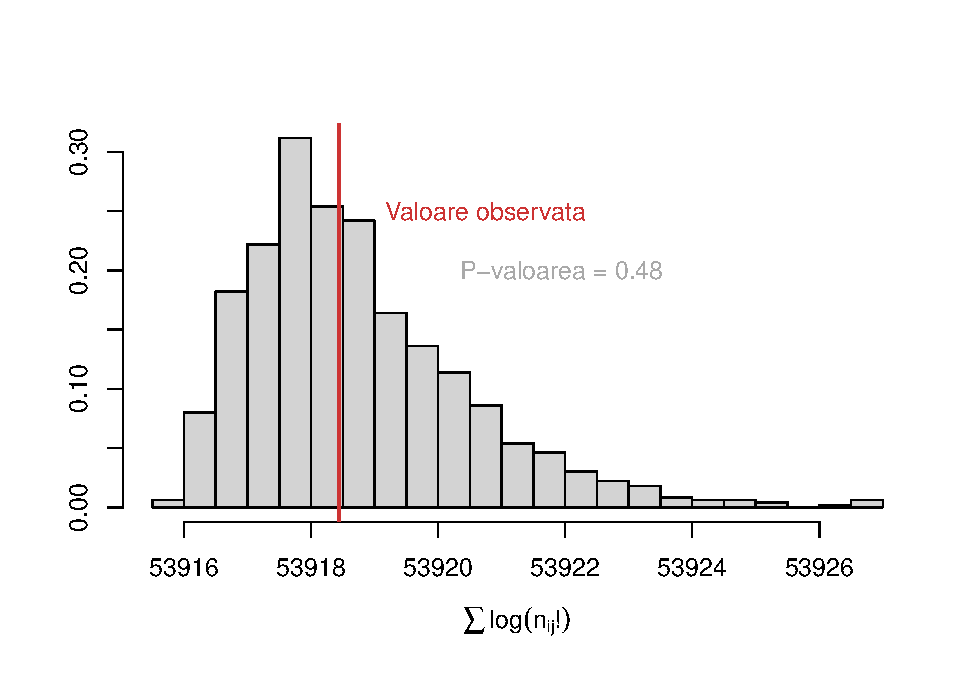
\includegraphics[width=0.8\linewidth]{Lab_5_files/figure-latex/unnamed-chunk-63-1} \end{center}

Același rezultat îl obținem și dacă folosim funcția
\texttt{fisher.test()} din R (care este mai rapidă):

\begin{Shaded}
\begin{Highlighting}[]
\KeywordTok{fisher.test}\NormalTok{(matAA_observed, }\DataTypeTok{simulate.p.value =} \OtherTok{TRUE}\NormalTok{, }\DataTypeTok{B =} \DecValTok{1000}\NormalTok{)}

\NormalTok{    Fisher}\StringTok{'s Exact Test for Count Data with simulated p-value (based}
\StringTok{    on 1000 replicates)}

\StringTok{data:  matAA_observed}
\StringTok{p-value = 0.4835}
\StringTok{alternative hypothesis: two.sided}
\end{Highlighting}
\end{Shaded}

\renewcommand\refname{Referințe}
\bibliography{references/Biostat2018ref.bib}


\end{document}
